\documentclass{llncs}

\usepackage{wrapfig}
\usepackage{amssymb,amsmath,mathtools}
\usepackage{cmll}
\usepackage{stmaryrd}
\usepackage{todonotes}
\usepackage{mathpartir}
\usepackage{hyperref}
\usepackage{mdframed}
\usepackage{thmtools, thm-restate}
\usepackage{enumitem}
\usepackage{minted}

%% This renames Barr's \to to \mto.  This allows us to use \to for imp
%% and \mto for a inline morphism.
\let\mto\to
\let\to\relax
\newcommand{\to}{\rightarrow}

% Commands that are useful for writing about type theory and programming language design.
%% \newcommand{\case}[4]{\text{case}\ #1\ \text{of}\ #2\text{.}#3\text{,}#2\text{.}#4}
\newcommand{\interp}[1]{\llbracket #1 \rrbracket}
\newcommand{\normto}[0]{\rightsquigarrow^{!}}
\newcommand{\join}[0]{\downarrow}
\newcommand{\redto}[0]{\rightsquigarrow}
\newcommand{\nat}[0]{\mathbb{N}}
\newcommand{\fun}[2]{\lambda #1.#2}
\newcommand{\CRI}[0]{\text{CR-Norm}}
\newcommand{\CRII}[0]{\text{CR-Pres}}
\newcommand{\CRIII}[0]{\text{CR-Prog}}
\newcommand{\subexp}[0]{\sqsubseteq}
%% Must include \usepackage{mathrsfs} for this to work.
\newcommand{\powerset}[0]{\mathscr{P}}

\date{}

% Cat commands.
\newcommand{\Four}[0]{\mathsf{4}}
\newcommand{\cat}[1]{\mathcal{#1}}
\newcommand{\catop}[1]{\cat{#1}^{\mathsf{op}}}
\newcommand{\Hom}[3]{\mathsf{Hom}_{\cat{#1}}(#2,#3)}
\newcommand{\limp}[0]{\multimap}
\newcommand{\dial}[1]{\mathsf{Dial_{#1}}(\mathsf{Sets})}
\newcommand{\dcSets}[1]{\mathsf{DC_{#1}}(\mathsf{Sets})}
\newcommand{\sets}[0]{\mathsf{Sets}}
\newcommand{\obj}[1]{\mathsf{Obj}(#1)}
\newcommand{\mor}[1]{\mathsf{Mor(#1)}}
\newcommand{\id}[0]{\mathsf{id}}
\newcommand{\lett}[0]{\mathsf{let}\,}
\newcommand{\inn}[0]{\,\mathsf{in}\,}
\newcommand{\cur}[1]{\mathsf{cur}(#1)}
\newcommand{\curi}[1]{\mathsf{cur}^{-1}(#1)}

\newenvironment{changemargin}[2]{%
  \begin{list}{}{%
    \setlength{\topsep}{0pt}%
    \setlength{\leftmargin}{#1}%
    \setlength{\rightmargin}{#2}%
    \setlength{\listparindent}{\parindent}%
    \setlength{\itemindent}{\parindent}%
    \setlength{\parsep}{\parskip}%
  }%
  \item[]}{\end{list}}

%% Ott
%% \input{aterms-ott}
% generated by Ott 0.25 from: attack-trees/attack-trees.ott
\newcommand{\ATermsdrule}[4][]{{\displaystyle\frac{\begin{array}{l}#2\end{array}}{#3}\quad\ATermsdrulename{#4}}}
\newcommand{\ATermsusedrule}[1]{\[#1\]}
\newcommand{\ATermspremise}[1]{ #1 \\}
\newenvironment{ATermsdefnblock}[3][]{ \framebox{\mbox{#2}} \quad #3 \\[0pt]}{}
\newenvironment{ATermsfundefnblock}[3][]{ \framebox{\mbox{#2}} \quad #3 \\[0pt]\begin{displaymath}\begin{array}{l}}{\end{array}\end{displaymath}}
\newcommand{\ATermsfunclause}[2]{ #1 \equiv #2 \\}
\newcommand{\ATermsnt}[1]{\mathit{#1}}
\newcommand{\ATermsmv}[1]{\mathit{#1}}
\newcommand{\ATermskw}[1]{\mathbf{#1}}
\newcommand{\ATermssym}[1]{#1}
\newcommand{\ATermscom}[1]{\text{#1}}
\newcommand{\ATermsdrulename}[1]{\textsc{#1}}
\newcommand{\ATermscomplu}[5]{\overline{#1}^{\,#2\in #3 #4 #5}}
\newcommand{\ATermscompu}[3]{\overline{#1}^{\,#2<#3}}
\newcommand{\ATermscomp}[2]{\overline{#1}^{\,#2}}
\newcommand{\ATermsgrammartabular}[1]{\begin{supertabular}{llcllllll}#1\end{supertabular}}
\newcommand{\ATermsmetavartabular}[1]{\begin{supertabular}{ll}#1\end{supertabular}}
\newcommand{\ATermsrulehead}[3]{$#1$ & & $#2$ & & & \multicolumn{2}{l}{#3}}
\newcommand{\ATermsprodline}[6]{& & $#1$ & $#2$ & $#3 #4$ & $#5$ & $#6$}
\newcommand{\ATermsfirstprodline}[6]{\ATermsprodline{#1}{#2}{#3}{#4}{#5}{#6}}
\newcommand{\ATermslongprodline}[2]{& & $#1$ & \multicolumn{4}{l}{$#2$}}
\newcommand{\ATermsfirstlongprodline}[2]{\ATermslongprodline{#1}{#2}}
\newcommand{\ATermsbindspecprodline}[6]{\ATermsprodline{#1}{#2}{#3}{#4}{#5}{#6}}
\newcommand{\ATermsprodnewline}{\\}
\newcommand{\ATermsinterrule}{\\[5.0mm]}
\newcommand{\ATermsafterlastrule}{\\}
\usepackage{cmll}
                 \usepackage{relsize} 
\newcommand{\ATermsmetavars}{
\ATermsmetavartabular{
 $ \ATermsmv{termvar} ,\, \ATermsmv{x} ,\, \ATermsmv{y} ,\, \ATermsmv{z} ,\, \ATermsmv{f} $ &  \\
 $ \ATermsmv{baseAttackVars} ,\, \ATermsmv{a} ,\, \ATermsmv{b} ,\, \ATermsmv{c} ,\, d ,\, \ATermsmv{N} $ &  \\
 $ \ATermsmv{baseAttackTVars} ,\, \ATermsmv{n} $ &  \\
 $ \ATermsmv{index} ,\, \ATermsmv{i} ,\, \ATermsmv{j} ,\, \ATermsmv{k} $ &  \\
}}

\newcommand{\ATermsA}{
\ATermsrulehead{\ATermsnt{A}  ,\ \ATermsnt{B}  ,\ \ATermsnt{C}  ,\ \ATermsnt{E}  ,\ \ATermsnt{F}  ,\ D  ,\ \ATermsnt{T}  ,\ \ATermsnt{S}}{::=}{}\ATermsprodnewline
\ATermsfirstprodline{|}{\ATermsmv{b}}{}{}{}{}\ATermsprodnewline
\ATermsprodline{|}{ \mathsf{AND}( \ATermsnt{A} , \ATermsnt{B} ) }{}{}{}{}\ATermsprodnewline
\ATermsprodline{|}{ \mathsf{SEQ}( \ATermsnt{A} , \ATermsnt{B} ) }{}{}{}{}\ATermsprodnewline
\ATermsprodline{|}{ \mathsf{OR}( \ATermsnt{A} , \ATermsnt{B} ) }{}{}{}{}\ATermsprodnewline
\ATermsprodline{|}{\ATermssym{(}  \ATermsnt{A}  \ATermssym{)}}{}{}{}{}\ATermsprodnewline
\ATermsprodline{|}{ \ATermsnt{A} }{}{}{}{}}

\newcommand{\ATermsterminals}{
\ATermsrulehead{\ATermsnt{terminals}}{::=}{}\ATermsprodnewline
\ATermsfirstprodline{|}{ \odot }{}{}{}{}\ATermsprodnewline
\ATermsprodline{|}{ \oplus }{}{}{}{}\ATermsprodnewline
\ATermsprodline{|}{ \rhd }{}{}{}{}\ATermsprodnewline
\ATermsprodline{|}{ \sqcup }{}{}{}{}\ATermsprodnewline
\ATermsprodline{|}{ \rightharpoonup }{}{}{}{}\ATermsprodnewline
\ATermsprodline{|}{ \leftharpoonup }{}{}{}{}\ATermsprodnewline
\ATermsprodline{|}{ \multimap }{}{}{}{}\ATermsprodnewline
\ATermsprodline{|}{ \multimapboth }{}{}{}{}\ATermsprodnewline
\ATermsprodline{|}{ \vdash }{}{}{}{}\ATermsprodnewline
\ATermsprodline{|}{ \not \vdash }{}{}{}{}\ATermsprodnewline
\ATermsprodline{|}{ \mathsf{succ} }{}{}{}{}\ATermsprodnewline
\ATermsprodline{|}{ \approx }{}{}{}{}\ATermsprodnewline
\ATermsprodline{|}{ \sim_U }{}{}{}{}\ATermsprodnewline
\ATermsprodline{|}{ \in }{}{}{}{}\ATermsprodnewline
\ATermsprodline{|}{ \rightsquigarrow }{}{}{}{}\ATermsprodnewline
\ATermsprodline{|}{ \rightsquigarrow_\copyright }{}{}{}{}\ATermsprodnewline
\ATermsprodline{|}{ \rightsquigarrow^*_\copyright }{}{}{}{}\ATermsprodnewline
\ATermsprodline{|}{ \leftsquigarrow }{}{}{}{}\ATermsprodnewline
\ATermsprodline{|}{ \rightsquigarrow^{\hspace{-1.5px}*} }{}{}{}{}\ATermsprodnewline
\ATermsprodline{|}{ \prescript{*\hspace{-2px} }{}{\leftsquigarrow} }{}{}{}{}\ATermsprodnewline
\ATermsprodline{|}{ \mathsf{box} }{}{}{}{}\ATermsprodnewline
\ATermsprodline{|}{ \mathsf{unbox} }{}{}{}{}\ATermsprodnewline
\ATermsprodline{|}{ \mathsf{fst} }{}{}{}{}\ATermsprodnewline
\ATermsprodline{|}{ \mathsf{snd} }{}{}{}{}\ATermsprodnewline
\ATermsprodline{|}{ \neq }{}{}{}{}\ATermsprodnewline
\ATermsprodline{|}{ \not\in }{}{}{}{}\ATermsprodnewline
\ATermsprodline{|}{ \simeq }{}{}{}{}}

\newcommand{\ATermsformula}{
\ATermsrulehead{\ATermsnt{formula}}{::=}{}\ATermsprodnewline
\ATermsfirstprodline{|}{\ATermsnt{judgement}}{}{}{}{}\ATermsprodnewline
\ATermsprodline{|}{ \ATermsnt{formula_{{\mathrm{1}}}}  \quad  \ATermsnt{formula_{{\mathrm{2}}}} }{}{}{}{}\ATermsprodnewline
\ATermsprodline{|}{ \ATermsnt{formula} } {\textsf{S}}{}{}{}\ATermsprodnewline
\ATermsprodline{|}{\ATermsnt{T_{{\mathrm{1}}}}  \rightsquigarrow  \ATermsnt{T_{{\mathrm{2}}}}} {\textsf{M}}{}{}{}\ATermsprodnewline
\ATermsprodline{|}{\ATermsnt{T_{{\mathrm{1}}}}  \rightsquigarrow_\copyright  \ATermsnt{T_{{\mathrm{2}}}}} {\textsf{M}}{}{}{}\ATermsprodnewline
\ATermsprodline{|}{\ATermsnt{T_{{\mathrm{1}}}}  \rightsquigarrow^*_\copyright  \ATermsnt{T_{{\mathrm{2}}}}} {\textsf{M}}{}{}{}\ATermsprodnewline
\ATermsprodline{|}{\ATermsnt{T_{{\mathrm{1}}}}  \leftsquigarrow  \ATermsnt{T_{{\mathrm{2}}}}} {\textsf{M}}{}{}{}\ATermsprodnewline
\ATermsprodline{|}{\ATermsnt{T_{{\mathrm{1}}}}  \rightsquigarrow^{\hspace{-1.5px}*}  \ATermsnt{T_{{\mathrm{2}}}}} {\textsf{M}}{}{}{}\ATermsprodnewline
\ATermsprodline{|}{\ATermsnt{T_{{\mathrm{1}}}}  \prescript{*\hspace{-2px} }{}{\leftsquigarrow}  \ATermsnt{T_{{\mathrm{2}}}}} {\textsf{M}}{}{}{}\ATermsprodnewline
\ATermsprodline{|}{\ATermsnt{T_{{\mathrm{1}}}}  \simeq  \ATermsnt{T_{{\mathrm{2}}}}} {\textsf{M}}{}{}{}\ATermsprodnewline
\ATermsprodline{|}{ \ATermsnt{T_{{\mathrm{1}}}}  \curlyveedownarrow  \ATermsnt{T_{{\mathrm{2}}}} } {\textsf{M}}{}{}{}}

\newcommand{\ATermsTyping}{
\ATermsrulehead{\ATermsnt{Typing}}{::=}{}\ATermsprodnewline
\ATermsfirstprodline{|}{ \ATermsnt{T_{{\mathrm{1}}}}  \approx  \ATermsnt{T_{{\mathrm{2}}}} }{}{}{}{}}

\newcommand{\ATermsjudgement}{
\ATermsrulehead{\ATermsnt{judgement}}{::=}{}\ATermsprodnewline
\ATermsfirstprodline{|}{\ATermsnt{Typing}}{}{}{}{}}

\newcommand{\ATermsuserXXsyntax}{
\ATermsrulehead{\ATermsnt{user\_syntax}}{::=}{}\ATermsprodnewline
\ATermsfirstprodline{|}{\ATermsmv{termvar}}{}{}{}{}\ATermsprodnewline
\ATermsprodline{|}{\ATermsmv{baseAttackVars}}{}{}{}{}\ATermsprodnewline
\ATermsprodline{|}{\ATermsmv{baseAttackTVars}}{}{}{}{}\ATermsprodnewline
\ATermsprodline{|}{\ATermsmv{index}}{}{}{}{}\ATermsprodnewline
\ATermsprodline{|}{\ATermsnt{A}}{}{}{}{}\ATermsprodnewline
\ATermsprodline{|}{\ATermsnt{terminals}}{}{}{}{}\ATermsprodnewline
\ATermsprodline{|}{\ATermsnt{formula}}{}{}{}{}}

\newcommand{\ATermsgrammar}{\ATermsgrammartabular{
\ATermsA\ATermsinterrule
\ATermsterminals\ATermsinterrule
\ATermsformula\ATermsinterrule
\ATermsTyping\ATermsinterrule
\ATermsjudgement\ATermsinterrule
\ATermsuserXXsyntax\ATermsafterlastrule
}}

% defnss
% defns Typing
%% defn eqat

\newcommand{\ATermsdefneqat}[1]{\begin{ATermsdefnblock}[#1]{$ \ATermsnt{T_{{\mathrm{1}}}}  \approx  \ATermsnt{T_{{\mathrm{2}}}} $}{}
\end{ATermsdefnblock}}


\newcommand{\ATermsdefnsTyping}{
\ATermsdefneqat{}}

\newcommand{\ATermsdefnss}{
\ATermsdefnsTyping
}

\newcommand{\ATermsall}{\ATermsmetavars\\[0pt]
\ATermsgrammar\\[5.0mm]
\ATermsdefnss}



\begin{document}

\title{On Linear Logic, Functional Programming, and Attack Trees}

\author{Harley Eades III\inst{1} \and Jiaming Jiang\inst{2} \and Aubrey Bryant\inst{3}}

\institute{Computer Science, Augusta University, \href{mailto:harley.eades@gmail.com}{harley.eades@gmail.com}
\and
Computer Science, North Carolina State University
\and
Computer Science, Augusta University}

\maketitle

\begin{abstract}
  This paper has two main contributions. The first is a new linear
  logical semantics of causal attack trees in four-valued truth
  tables.  Our semantics is very simple and expressive, supporting
  specializations, and supports the \emph{ideal} semantics of causal
  attack trees, and partially supporting the \emph{filter} semantics
  of causal attack trees. Our second contribution is Lina, a new
  embedded, in Haskell, domain specific functional programming
  language for conducting threat analysis using attack trees.  Lina
  has many benefits over existing tools; for example, Lina allows one
  to specify attack trees very abstractly, which provides the ability
  to develop libraries of attack trees, furthermore, Lina is
  compositional, allowing one to break down complex attack trees into
  smaller ones that can be reasoned about and analyzed incrementally.
  Furthermore, Lina supports automatically proving properties of
  attack trees, such as equivalences and specializations, using Maude
  and the semantics introduced in this paper.
\end{abstract}

\section{Introduction}
\label{sec:introduction}
%% \input{intro-output}
%% - Better understanding the theory of attack trees
%% - Specializations using implication
%% - Lina!!
Attack trees are perhaps the most popular graphical model used to
conduct threat analysis of both physical and virtual secure
systems. They were made popular by Bruce Schneier in the late nineties
\cite{Schneier:1999}.  In those early years attack trees were studied
and used as a syntactic tool to help guide analysis.  However, as
systems grew more complex the need for a semantics of attack trees
become apparent; after all, without a proper semantics how can we
safely manipulate attack trees, extend their expressivity, or compare
them?

A number of different models of attack trees have been proposed: a
model in Boolean algebras
\cite{Kordy:2014,Kordy:2012,Pietre-Cambacedes:2010}, series-parallel
pomsets \cite{Mauw:2006}, Petri nets \cite{McDermott:2001}, and tree
automata \cite{Camtepe:2007}.  There have also been various
extensions, such as, adding sequential composition \cite{Jhawar:2015},
and defense nodes \cite{Kordy:2011,Kordy:2012}.  All of these models
and extensions have their benefits, but at the heart of them all is
logic.

The model in Boolean algebras was the first and most elegant model of
attack trees, but it failed to capture the process aspect of attack
trees, that is, the fact that base attacks are actual processes that
need to be carried out, and the branching nodes compose these
processes in different ways.  Thus, the community moved towards models
of resources like parallel-series pomsets, Petri nets, and automata.
However, the complexity of these models increased, and hence,
comparing these models becomes difficult. Furthermore, this increased
complexity makes it hard to decide which to use and under which
circumstances.  This difficulty can be resolved by recovering the
elegant logical model of attack trees.

\textbf{Linear Logic.}  It is fitting that attack trees are the most
popular model used in threat analysis, because \emph{linear logic},
one of the most widely studied logics used to reason about resources,
is also an excellent candidate for modeling attack trees.  In fact,
Horne et al.\cite{horne2017semantics} has already produced a number of
interesting results.  Most importantly, they show that attack trees
can be modeled as formulas in linear logic, which then one can prove
properties between attack trees by proving implications between them.
Furthermore, by studying attack trees from a linear logical
perspective they introduce a new property between attack trees called
\emph{specializations}.  Prior to their paper the literature was
primarily concerned with equality between attack trees, but the
logical semantics of attack trees reveal how one can break these
equalities up into directional rewrite rules.  An attack tree is a
\emph{specialization} of another if the former is related to the later
via these rewrite rules.  The logical semantics model the rewrite
rules as implications.

This paper has two main contributions. The first is a new simple
linear logical semantics of causal attack trees -- attack trees with
sequential composition -- in four-valued truth tables.  It comes in
two flavors: the ideal quaternary logic
(Section~\ref{subsec:the_ideal_quaternary_semantics}) and the
filterish quaternary logic
(Section~\ref{subsec:the_filterish_quaternary_semantics}).  These two
types of semantics correspond to truth table semantics for Horne et
al.'s\cite{horne2017semantics} \emph{ideal} and \emph{filter}
semantics of causal attack trees.

\textbf{Functional Programming.} Our second contribution is Lina, a
new domain specific functional programming language for conducting
threat analysis using attack trees.  Consider the example attack trees
in Fig.~\ref{fig:atm-tree}.
\begin{figure}
  \vspace{-10px}
  \begin{tabular}{|l|l|}
    \hline
    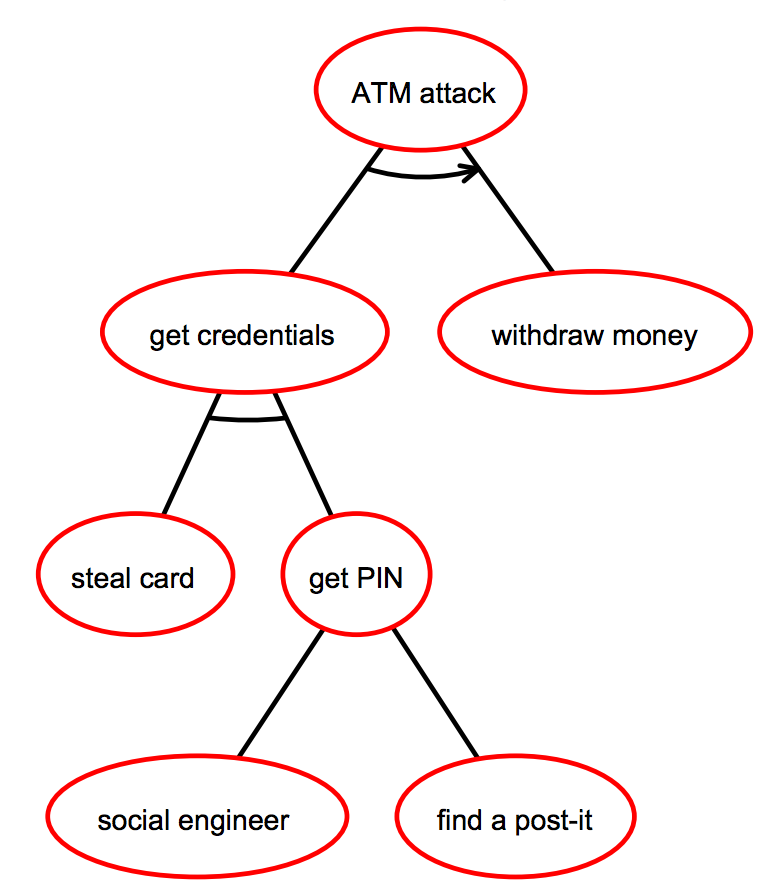
\includegraphics[scale=0.230]{ATM-Tree1}
    &
    \begin{tabular}{l}      
      \begin{minipage}{2.2in}
        \vspace{-200px}
        \begin{minted}[fontsize=\footnotesize]{haskell}
seq_node "ATM attack"
  (and_node "get credentials"
    (base_na "steal card")
    (or_node "get PIN"
      (base_na "social engineer")
      (base_na "find a post-it")))
  (base_na "withdraw money")
        \end{minted}        
      \end{minipage}
    \end{tabular}\\
    \hline
  \end{tabular}
  \\[5px]
  \begin{tabular}{|c|l|}
    \hline
    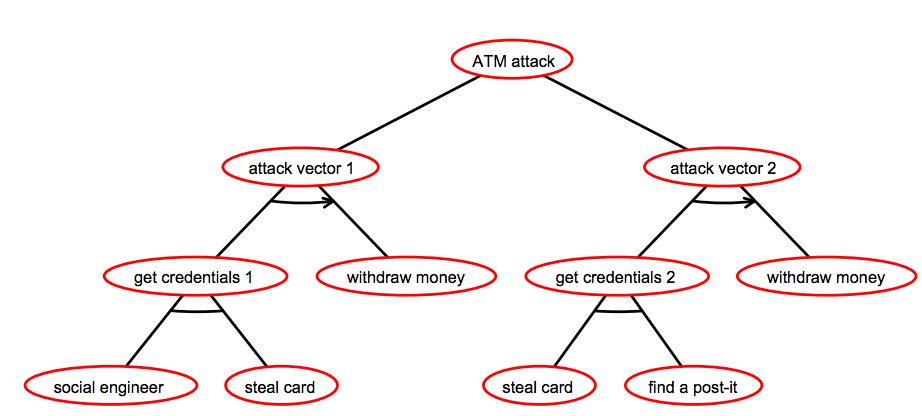
\includegraphics[scale=0.37]{ATM-Tree2}
    \\
    \hline
    \begin{tabular}{l}
      \begin{minipage}{2.5in}
        \vspace{4px}
    \begin{minted}[fontsize=\footnotesize]{haskell}
or_node "ATM attack"
   (seq_node "attack vector 1"
     (and_node "get credentials 1"
       (base_na "social engineer")
       (base_na "steal card"))
     (base_na "withdraw money"))
   (seq_node "attack vector 2"
     (and_node "get credentials 2"
       (base_na "steal card")
       (base_na "find a post-it"))
     (base_na "withdraw money"))
    \end{minted}
    \vspace{4px}
    \end{minipage}
    \end{tabular}\\
    \hline
  \end{tabular}  
  \label{fig:atm-tree}
  \caption{Attack Trees for an ATM attack from Figure~1 and Figure~2 of Kordy et
    al.~\cite{Kordy2017} and their corresponding Lina scripts.}
\vspace{-15px}  
\end{figure}
Both of these contain actual Lina programs for each of the
corresponding attack trees; in fact, every example in this paper is a
Lina program. Lina supports causal attack trees with attributes or
without; thus, there are two types of base attacks: \underline{base}
attacks \underline{w}ith \underline{a}ttributes, denoted
\verb!base_wa!, and \underline{base} attacks \text{w}ith
\underline{n}o \underline{a}ttributes, denoted \verb!base_na!; an
example usage of the former can be found in
Fig.~\ref{fig:vehicle_attack}.  Lina is designed to be extremely
simple, and to reflect the typical pseudocode found throughout the
literature.  However, Lina is more than just a simple definitional
language.

Lina is an embedded domain-specific programming language whose host
language is the Haskell programming language \cite{jones2003haskell}.
So, why Haskell?  As security researchers and professionals, we are in
the business of verifying the correctness of various systems. Thus, we
should be taking advantage of verification tools to insure that our
constructions, tools, and analysis are correct.  By embedding Lina
into Haskell, we are able to take advantage of cutting-edge
verification tools while conducting threat analysis.  For example,
right out the box Lina supports property-based randomized testing
using QuickCheck \cite{Claessen:2011:QLT:1988042.1988046}, and
refinement types in Liquid Haskell
\cite{Vazou:2014:RTH:2692915.2628161} to verify properties of our
attack trees or the attribute domains used while analyzing attack
trees.  Furthermore, Haskell's advanced type system helps catch bugs
while we develop our attack trees and their attribute domains as a
side-effect of type checking.  Finally, functional programs are short,
but not obfuscated, and hence allow for very compact and trustworthy
programs.

That being said, we are designing Lina so that it can be used with
very little Haskell experience.  It is our hope that one will be able
to make use of Lina without knowing Haskell, and we plan to develop
new tooling to support this.

Lina approaches threat analysis from a programming language
perspective, leading to a number of new advances.  First, as
Gadyatskaya and Trujillo-Rasua \cite{10.1007/978-3-319-74860-3_9}
argue, as a community we need to start building more automated means
of conducting threat analysis, and there is no better way to build or
connect automated tools than a programming language.  Lina is perfect
as a target for new tools, and it can be connected to existing tools
fairly easily.  In fact, Lina already supports automation using the
automatic rewrite system Maude \cite{clavel2005maude}; for example,
the two attack trees in Fig.~\ref{fig:atm-tree} can be automatically
proven equivalent to each other in Lina.  This is similar to Kordy's
\cite{Kordy2017} SPTool, but Lina goes further and supports more than
one backend rewrite system; for example, Lina is the first tool to
support automatically proving specializations of attack trees.  The
user can choose which backend they wish to use.

%%% Local Variables: 
%%% mode: latex
%%% TeX-master: main.tex
%%% End: 


\vspace{-7px}
\section{Causal Attack Trees}
\label{sec:causal_attack_trees}
%% \input{attack-trees-output}
We begin by introducing causal attack trees.  This formulation of
attack trees was first proposed by Jhawar et al. \cite{Jhawar:2015},
where they called them SAND attack trees, however sequential
composition does not always maintain the same properties as
conjunction; for example, classically it is a self dual operator.
Thus, we follow Horne et al.'s lead \cite{horne2017semantics} and call
them causal attack trees.
\begin{definition}
  \label{def:atrees}
  Suppose $\mathbb{B}$ is a set of base attacks whose elements are
  denoted by $\ATermsmv{b}$.  Then an \textbf{attack tree} is defined by
  the following grammar:
  \[
  \begin{array}{lll}
    \ATermsnt{A},\ATermsnt{B},\ATermsnt{C},\ATermsnt{T} := \ATermsmv{b} \mid  \mathsf{OR}( \ATermsnt{A} , \ATermsnt{B} )  \mid  \mathsf{AND}( \ATermsnt{A} , \ATermsnt{B} )  \mid  \mathsf{SEQ}( \ATermsnt{A} , \ATermsnt{B} ) \\
  \end{array}
  \]
  \noindent
  Equivalence of attack trees, denoted by $ \ATermsnt{A}  \approx  \ATermsnt{B} $, is defined as
  follows:
  \begin{center}
    \begin{math} \footnotesize
      \begin{array}{|l|l|}
        \hline
        \begin{array}{lll}
            \mathsf{OR}( \ATermsnt{A} , \ATermsnt{A} )   \approx  \ATermsnt{A} \\
            \mathsf{OR}( \ATermsnt{A} , \ATermsnt{B} )   \approx   \mathsf{OR}( \ATermsnt{B} , \ATermsnt{A} )  \\
            \mathsf{AND}( \ATermsnt{A} , \ATermsnt{B} )   \approx   \mathsf{AND}( \ATermsnt{B} , \ATermsnt{A} )  \\
          \\\\
        \end{array}
        &
        \begin{array}{lll}          
            \mathsf{OR}(  \mathsf{OR}( \ATermsnt{A} , \ATermsnt{B} )  , \ATermsnt{C} )   \approx   \mathsf{OR}( \ATermsnt{A} ,  \mathsf{OR}( \ATermsnt{B} , \ATermsnt{C} )  )  \\
            \mathsf{AND}(  \mathsf{AND}( \ATermsnt{A} , \ATermsnt{B} )  , \ATermsnt{C} )   \approx   \mathsf{AND}( \ATermsnt{A} ,  \mathsf{AND}( \ATermsnt{B} , \ATermsnt{C} )  )  \\
            \mathsf{SEQ}(  \mathsf{SEQ}( \ATermsnt{A} , \ATermsnt{B} )  , \ATermsnt{C} )   \approx   \mathsf{SEQ}( \ATermsnt{A} ,  \mathsf{SEQ}( \ATermsnt{B} , \ATermsnt{C} )  )  \\                
            \mathsf{AND}( \ATermsnt{A} ,  \mathsf{OR}( \ATermsnt{B} , \ATermsnt{C} )  )   \approx   \mathsf{OR}(  \mathsf{AND}( \ATermsnt{A} , \ATermsnt{B} )  ,  \mathsf{AND}( \ATermsnt{A} , \ATermsnt{C} )  )  \\
            \mathsf{SEQ}( \ATermsnt{A} ,  \mathsf{OR}( \ATermsnt{B} , \ATermsnt{C} )  )   \approx   \mathsf{OR}(  \mathsf{SEQ}( \ATermsnt{A} , \ATermsnt{B} )  ,  \mathsf{SEQ}( \ATermsnt{A} , \ATermsnt{C} )  )  \\
        \end{array}\\
        \hline
      \end{array}
    \end{math}  
  \end{center}
\end{definition}
Throughout the sequel we will show that the previous rules are sound
with respect to our new model, but just as Horne et
al. \cite{horne2017semantics} did, we will then show that there are
properties of attack trees that these rules do not support, but our
semantics allows.

%%% Local Variables: 
%%% mode: latex
%%% TeX-master: main.tex
%%% End: 

% section causal_attack_trees (end)

\vspace{-7px}
\section{A Quaternary Semantics for Causal Attack Trees}
\label{sec:a_quaternary_semantics_for_causal_attack_trees}
%% \newcommand{\forth}{\frac{1}{4}}
\newcommand{\half}{\frac{1}{2}}

Kordy et al.~\cite{Kordy:2012} gave a very elegant and simple
semantics of attack-defense trees in boolean algebras.  Unfortunately,
while their semantics is elegant it does not capture the resource
aspect of attack trees, it allows contraction, and it does not provide
a means to model sequential conjunction.  In this section we give a
semantics of attack trees in the spirit of Kordy et al.'s using a four
valued logic.

The propositional variables of our ternary logic, denoted by $A$, $B$,
$C$, and $D$, range over the set $\mathsf{4} = \{0, \forth, \half,
1\}$.  We think of $0$ and $1$ as we usually do in boolean algebras,
but we think of $\forth$ and $\half$ as intermediate values that can
be used to break various structural rules.  In particular we will use
these values to prevent exchange for sequential conjunction from
holding, and contraction from holding for parallel and sequential
conjunction.
\begin{definition}
  \label{def:logical-connectives}
  The logical connectives of our four valued logic are defined as
  follows:
  \begin{itemize}
  \item[] Parallel and Sequential Conjunction:
    \begin{center}
      \begin{math}
        \setlength{\arraycolsep}{10px}
        \begin{array}{lll}
          \begin{array}{lll}
            A \odot_4 B = 1,\\
            \,\,\,\,\,\,\,\text{where neither $A$ nor $B$ are $0$}\\
          A \odot_4 B = 0, \text{otherwise}\\
          \\
        \end{array}
        &
        \begin{array}{lll}          
          A \rhd_4 B = 1,\\
          \,\,\,\,\,\,\,\text{where } A \in \{\half, 1\} \text{ and } B \neq 0\\
          \forth \rhd_4 B = \forth, \text{where $B \neq 0$}\\[2px]         
          A \rhd_4 B = 0, \text{otherwise}
        \end{array}
        \end{array}
      \end{math}
    \end{center}
  \item[] Choice: $A \sqcup_4 B = \mathsf{max}(A,B)$    
  \end{itemize}
\end{definition}
These definitions are carefully crafted to satisfy the necessary
properties to model attack trees.  Comparing these definitions with
Kordy et al.'s~\cite{Kordy:2012} work we can see that choice is
defined similarly, but parallel conjunction is not a product --
ordinary conjunction -- but rather a linear tensor product, and
sequential conjunction is not actually definable in a boolean algebra,
and hence, makes heavy use of the intermediate values to insure that
neither exchange nor contraction hold.  The following results solidify
these claims.

We use the usual notion of equivalence between propositions, that is,
propositions $\phi$ and $\psi$ are considered equivalent, denoted by
$\phi \equiv \psi$, if and only if they have the same truth tables. In
order to model attack trees the previously defined logical connectives
must satisfy the appropriate equivalences corresponding to the
equations between attack trees.  These equivalences are all proven by
the following results.
\begin{lemma}[Properties of the Attack Tree Operators in the Quaternary Semantics]
  \label{lemma:props_atree_ops_quaternary-semantics}
  \begin{itemize}
  \item[] (Symmetry) For any $A$ and $B$, $A \bullet B \equiv B \bullet A$, for $\bullet \in \{\odot_4, \sqcup_4\}$.\\[-5px]
  \item[] (Symmetry for Sequential Conjunction) It is not the case that, for any $A$ and $B$, $A \rhd_4 B \equiv B \rhd_4 A$.\\[-5px]
  \item[] (Associativity) For any $A$, $B$, and $C$, $(A \bullet B) \bullet C \equiv A \bullet (B \bullet C)$, for $\bullet \in \{\odot_4, \rhd_4, \sqcup_4\}$.\\[-5px]
  \item[] (Contraction for Parallel and Sequential Conjunction) It is not the case that for any $A$, $A \bullet A \equiv A$, for $\bullet \in \{\odot_4, \rhd_4\}$.\\[-5px]
  \item[] (Contraction for Choice) For any $A$, $A \sqcup_4 A \equiv_4 A$\\[-5px]
  \item[] (Left Distributive Law) For any $A$, $B$, and $C$, $A \bullet (B \sqcup_4 C) \equiv (A \bullet B) \sqcup_4 (A \bullet C)$, for $\bullet \in \{\odot_4, \rhd_4\}$.\\[-5px]
  \item[] (Right Distributive Law) For any $A$, $B$, and $C$, $(A \sqcup_4 B) \bullet C \equiv (A \bullet C) \sqcup_4 (B \bullet C)$, for $\bullet \in \{\odot_4, \rhd_4\}$.\\
  \end{itemize}
\end{lemma}
\begin{proof}
  Symmetry, associativity, contraction for choice, and the
  distributive laws for each operator hold by simply comparing truth
  tables.  As for contraction for parallel conjunction, suppose $A =
  \forth$.  Then by definition $A \odot_4 A = 1$, but $\forth$ is not
  $1$.  Contraction for sequential conjunction also fails, suppose $A
  = \half$.  Then by definition $A \rhd_4 A = 1$, but $\half$ is not
  $1$.  Similarly, symmetry fails for sequential conjunction. Suppose
  $A = \forth$ and $B = \half$.  Then $A \rhd_4 B = \forth$, but $B
  \rhd_4 A = 1$.
\end{proof}

At this point it is quite easy to model attack trees as formulas.  The
following defines their interpretation.
\begin{definition}
  \label{def:interp-aterms-ternary}
  Suppose $\mathbb{B}$ is some set of base attacks, and $\nu :
  \mathbb{B} \mto \mathsf{PVar}$ is an assignment of base attacks to
  propositional variables.  Then we define the interpretation of
  $\mathsf{ATerms}$ to propositions as follows:
  \begin{center}
    \begin{math}
      \setlength{\arraycolsep}{5px}
      \begin{array}{lll}
        \begin{array}{lll}
          \interp{[[b]] \in \mathbb{B}} & = & \nu([[b]])\\
          \interp{[[AND T1 T2]]} & = & \interp{[[T1]]} \odot_4 \interp{[[T2]]}\\
        \end{array}
        &
        \begin{array}{lll}
          \interp{[[SAND T1 T2]]} & = & \interp{[[T1]]} \rhd_4 \interp{[[T2]]}\\
          \interp{[[OR T1 T2]]} & = & \interp{[[T1]]} \sqcup_4 \interp{[[T2]]}\\
        \end{array}
      \end{array}
    \end{math}
  \end{center}
\end{definition}
We can use this semantics to prove equivalences between attack trees.
\begin{lemma}[Equivalence of Attack Trees in the Ternary Semantics]
  \label{lemma:equivalence_of_attack_trees}
  Suppose $\mathbb{B}$ is some set of base attacks, and $\nu :
  \mathbb{B} \mto \mathsf{PVar}$ is an assignment of base attacks to
  propositional variables.  Then for any attack trees $[[T1]]$ and
  $[[T2]]$, $[[T1 ~ T2]]$ if and only if $\interp{[[T1]]} \equiv \interp{[[T2]]}$.
\end{lemma}
\begin{proof}
  This proof holds by induction on the form of $[[T1 ~ T2]]$.
\end{proof}
This is a very simple and elegant semantics, but it also leads to a
more substantial theory.

%%% Local Variables: 
%%% mode: latex
%%% TeX-master: main.tex
%%% End: 

\newcommand{\forth}{\frac{1}{4}}
\newcommand{\half}{\frac{1}{2}}

Kordy et al.~\cite{Kordy:2012} gave a very elegant and simple
semantics of attack-defense trees in Boolean algebras.  Unfortunately,
while their semantics is elegant, it does not capture the resource
aspect of attack trees, it allows contraction, and it does not provide
a means to model sequential composition.  In this section we give a
semantics of attack trees in the spirit of Kordy et al.'s using a
four-valued logic.  This section was formally verified in the Agda
Proof Assistant~\cite{Norell:2009}\footnote{The formalization can be
  found at
  \url{https://github.com/MonoidalAttackTrees/ATLL-Formalization}}.

 We now give two types of quaternary semantics for casual attack
 trees.  We do this by defining two four-valued logics we call
 quaternary logics.  The propositional variables, elements of the set
 $\mathsf{PVar}$, of our quaternary logics, denoted by $P$, $Q$, $R$,
 and $S$, range over the set $\mathsf{4} = \{0, \forth, \half, 1\}$.
 We think of $0$ and $1$ as we usually do in Boolean algebras, but we
 think of $\forth$ and $\half$ as intermediate values that can be used
 to break various structural rules\footnote{Choosing $\forth$ and
   $\half$ as the symbols for the intermediate values was arbitrary,
   and one can choose any symbols at all for these two values and the
   semantics will still be correct.}.  In particular we will use these
 values to prevent exchange for sequential composition from holding,
 and contraction from holding for parallel and sequential composition.

We use the usual notion of equivalence between propositions; that is,
propositions $\phi$ and $\psi$ are considered equivalent, denoted by
$\phi \equiv \psi$, if and only if they have the same truth tables.
In addition, we define a notion of entailment for the quaternary
logics.  Denote by $P \leq_4 Q$ the usual natural number ordering
restricted to $\mathsf{4}$.  Then we have the following result
immediately.
\begin{lemma}[Entailment in the Quaternary Logics]
  \label{lemma:entailment_in_the_quaternary_semantics}
  $P \equiv Q$ if and only if $P \leq_4 Q$ and $Q \leq_4 P$
\end{lemma}
This result shows that we can break up the equivalence of attack trees
into directional properties captured here by entailments, and hence,
every equivalence proved throughout this section can also be used
directionally.

\subsection{The Ideal Quaternary Logic}
\label{subsec:the_ideal_quaternary_semantics}
%% \input{ideal-output}
The ideal semantics for casual attack trees was first proposed by
Horne et al.\cite{horne2017semantics}.  In this section we give a
simple truth table semantics that corresponds to their ideal semantics
within the ideal quaternary logic.

\begin{definition}
  \label{def:ideal-semantics}
  The logical connectives of the \emph{ideal quaternary logic} are
  defined as follows:\vspace{-5px}
  \begin{center}
    \begin{math}
      \setlength{\arraycolsep}{5px}
      \begin{array}{lll}
        \begin{array}{lll}
          \text{Parallel Composition:}\\
          \begin{array}{lll}
            P \odot_I Q = 1,\\
            \,\,\,\,\,\,\,\text{where neither $P$ nor $Q$ are $0$}\\
            P \odot_I Q = 0, \text{otherwise}\\\\\\
          \end{array}
        \end{array}
        &
        \begin{array}{lll}
          \text{Sequential Composition:}\\
          \begin{array}{lll}          
            P \rhd_I Q = \half,\\
            \,\,\,\,\,\,\,\text{where } P \in \{\half, 1\} \text{ and } Q \neq 0\\            
            P \rhd_I Q = \forth,\\
            \,\,\,\,\,\,\,\text{where } P = \forth \text{ and } Q \neq 0\\
            P \rhd_I Q = 0, \text{otherwise}\\
          \end{array}
        \end{array}
        \\[30px]
        \begin{array}{lll}
          \text{Choice:}\\    
          \begin{array}{lll}
            P \sqcup_I Q = \mathsf{max}(P,Q)
          \end{array}
        \end{array}
      \end{array}
    \end{math}
  \end{center}        
\end{definition}
These definitions are carefully crafted to satisfy the necessary
properties to model attack trees on the ideal semantics.  Comparing
these definitions with Kordy et al.'s~\cite{Kordy:2012} work we can
see that choice is defined similarly, but parallel composition is not
a product -- ordinary conjunction -- but rather a linear tensor
product. Sequential composition is not actually definable in a Boolean
algebra, and hence makes use of the intermediate values to insure that
neither exchange nor contraction hold.

In order to model attack trees, the previously defined logical
connectives must satisfy the appropriate equivalences corresponding to
the equations between attack trees.  We break these properties up into
the following lemmata.

\begin{lemma}[Basic Properties for Choice]
  \label{lemma:basic_properties_for_choice}
  The following properties hold:
  \begin{enumerate}
  \item $(P \sqcup_I Q) \equiv (Q \sqcup_I P)$\\[-5px]
  \item $((P \sqcup_I Q) \sqcup_I R) \equiv (P \sqcup_I (Q \sqcup_I R))$\\[-5px]
  \item $P \leq_4 (P \sqcup_I Q)$\\[-5px]
  \item $Q \leq_4 (P \sqcup_I Q)$\\[-5px]
  \item $\text{If }P \leq_4 R \text{ and } Q \leq_4 R \text{, then } (P \sqcup_I Q) \leq_4 R$\\[-5px]
  \item $\text{If }P \leq_4 R \text{ and } Q \leq_4 S \text{, then } (P \sqcup_I Q) \leq_4 (R \sqcup_I S)$
  \end{enumerate}
\end{lemma}
\begin{proof}
  Each of the properties hold by comparing truth tables.
\end{proof}
The previous lemma shows that choice has the same properties as
Boolean disjunction.  Hence, it is possible to show using these rules
that $P \sqcup_I P \equiv P$ which follows from properties three,
four, and five.
\begin{lemma}[Basic Properties for Parallel Composition]
  \label{lemma:basic_properties_for_parallel}
  The following properties hold:
  \begin{enumerate}
  \item $(P \odot_I P) \not\equiv P$\\[-5px]
  \item $(P \odot_I Q) \equiv (Q \odot_I P)$\\[-5px]
  \item $((P \odot_I Q) \odot_I R) \equiv (P \odot_I (Q \odot_I R))$\\[-5px]
  \item $(P \odot_I (Q \sqcup_I R)) \equiv ((P \odot_I Q) \sqcup_I (P \odot_I R))$\\[-5px]
  \item $\text{If }P \leq_4 R \text{ and } Q \leq_4 S \text{, then } (P \odot_I Q) \leq_4 (R \odot_I S)$
  \end{enumerate}
\end{lemma}
\begin{proof}
  We give the proof of property one.  The other properties hold by
  comparing truth tables.  Suppose $P = \half$, then $P \odot_I P =
  \half \odot_I \half = 1$, but $1$ is not $\half$.
\end{proof}
The previous lemma shows that sequential composition is a linear
tensor product.  In particular, the first property guarantees that
sequential composition does not contract parallel copies of attack
trees into a single attack tree.
\begin{lemma}[Basic Properties for Sequential Composition]
  \label{lemma:basic_properties_for_parallel}
  The following properties hold:
  \begin{enumerate}
  \item $(P \rhd_I P) \not\equiv P$\\[-5px]
  \item $(P \rhd_I Q) \not\equiv (Q \rhd_I P)$\\[-5px]
  \item $(P \rhd_I (Q \rhd_I R)) \equiv ((P \rhd_I Q) \rhd_I R)$\\[-5px]
  \item $(P \rhd_I (Q \sqcup_I R)) \equiv ((P \rhd_I Q) \sqcup_I (P \rhd_I R))$\\[-5px]
  \item $\text{If }P \leq_4 R \text{ and } Q \leq_4 S \text{, then } (P \rhd_I Q) \leq_4 (R \rhd_I S)$
  \end{enumerate}
\end{lemma}
\begin{proof}
  We give proofs for properties one and two, but the others hold by
  comparing truth tables.  As for property one, suppose $P = 1$, then
  $P \rhd_I P = 1 \rhd_I 1 = \half$, but $1$ is not $\half$.  Now for
  property two, suppose $P = 1$ and $Q = \forth$, then $P \rhd_I Q = 1
  \rhd_I \forth = \half$, but $Q \rhd_I P = \forth \rhd_I 1 = \forth$.
\end{proof}
This lemma is similar to the previous.  However, property two
guarantees that sequential composition is not commutative.
\begin{lemma}[The Ideal Properties]
  \label{lemma:the_ideal_properties}
  The following properties hold:
  \begin{enumerate}
  \item $((P \odot_I Q) \rhd_I (R \odot_I S)) \leq_4 ((P \rhd_I R) \odot_I (Q \rhd_I S))$\\[-5px]
  \item $((P \odot_I Q) \rhd_I R) \leq_4 (P \odot_I (Q \rhd_I R))$\\[-5px]
  \item $(P \rhd_I (Q \odot_I R) \leq_4 (Q \odot_I (P \rhd_I R))$\\[-5px]
  \item $(P \rhd_I Q) \leq_4 (P \odot_I Q)$
  \end{enumerate}
\end{lemma}
\begin{proof}
  Each property holds by comparing truth tables.
\end{proof}

At this point it is quite easy to model attack trees as formulas.  The
following defines their interpretation.
\begin{definition}
  \label{def:interp-aterms-quaternary}
  Suppose $\mathbb{B}$ is some set of base attacks, and $\nu :
  \mathbb{B} \mto \mathsf{PVar}$ is an assignment of base attacks to
  propositional variables.  Then we define the interpretation of
  attack trees to propositions as follows:
  \begin{center}
    \begin{math}
      \setlength{\arraycolsep}{5px}
      \begin{array}{lll}
        \begin{array}{lll}
          \interp{\ATermsmv{b} \in \mathbb{B}} & = & \nu(\ATermsmv{b})\\
          \interp{ \mathsf{AND}( \ATermsnt{A} , \ATermsnt{B} ) } & = & \interp{\ATermsnt{A}} \odot_I \interp{\ATermsnt{B}}
        \end{array}
        &
        \begin{array}{lll}
          \interp{ \mathsf{SEQ}( \ATermsnt{A} , \ATermsnt{B} ) } & = & \interp{\ATermsnt{A}} \rhd_I \interp{\ATermsnt{B}}\\
          \interp{ \mathsf{OR}( \ATermsnt{A} , \ATermsnt{B} ) } & = & \interp{\ATermsnt{A}} \sqcup_I \interp{\ATermsnt{B}}
        \end{array}
      \end{array}
    \end{math}
  \end{center}
\end{definition}
We can use this semantics to prove equivalences between attack trees.
\begin{lemma}[Equivalence of Attack Trees in the Ideal Quaternary Semantics]
  \label{lemma:equivalence_of_attack_trees}
  Suppose $\mathbb{B}$ is some set of base attacks, and $\nu :
  \mathbb{B} \mto \mathsf{PVar}$ is an assignment of base attacks to
  propositional variables.  Then for any attack trees $\ATermsnt{A}$ and
  $\ATermsnt{B}$, if $ \ATermsnt{A}  \approx  \ATermsnt{B} $, then $\interp{\ATermsnt{A}} \equiv
  \interp{\ATermsnt{B}}$.
\end{lemma}
\begin{proof}
  This proof holds by induction on the form of $ \ATermsnt{A}  \approx  \ATermsnt{B} $.
\end{proof}

%%% Local Variables: 
%%% mode: latex
%%% TeX-master: main.tex
%%% End: 

% subsection the_ideal_quaternary_semantics (end)

\subsection{The Filterish Quaternary Logic}
\label{subsec:the_filterish_quaternary_semantics}
%% \input{filter-output}
We now introduce the filterish semantics for casual attack trees.
This is a restricted notion of the filter semantics of Horne et
al.~\cite{horne2017semantics}.  We were unable to find a quaternary
semantics for the full filter semantics, because we obtained
contractions when attempting to satisfy the corresponding
specialization properties in the filter model.  We are unsure if these
contradictions arise due to the fact that the semantics proposed here
is intuitionistic while Horne et al.~\cite{horne2017semantics} use
classical logic, or if four values just are not enough, or if we just
have not been able to find it.

In this section we do as we did in the previous and define a
quaternary logic called the \emph{filterish quaternary logic}.
\begin{definition}
  \label{def:filterish-semantics}
  The logical connectives of the \emph{filterish quaternary logic} are
  defined as follows:\vspace{-5px}
  \begin{center}
    \begin{math}
      \setlength{\arraycolsep}{5px}
      \begin{array}{lll}
        \begin{array}{lll}
          \text{Parallel Composition:}\\
          \begin{array}{lll}
            P \odot_F Q = \half,\\
            \,\,\,\,\,\,\,\text{where neither $P$ nor $Q$ are $0$}\\
            P \odot_F Q = 0, \text{otherwise}\\\\\\
          \end{array}
        \end{array}
        &
        \begin{array}{lll}
          \text{Sequential Composition:}\\
          \begin{array}{lll}          
            P \rhd_F Q = 1,\\
            \,\,\,\,\,\,\,\text{where } P \in \{\half, 1\} \text{ and } Q \neq 0\\
            P \rhd_F Q = \forth,\\
            \,\,\,\,\,\,\,\text{where } P = \forth  \text{ and } Q \neq 0\\
            P \rhd_F Q = 0, \text{otherwise}
          \end{array}
        \end{array}
        \\[30px]
        \begin{array}{lll}
          \text{Choice:}\\    
          \begin{array}{lll}
            P \sqcup_F Q = \mathsf{max}(P,Q)
          \end{array}
        \end{array}
      \end{array}
    \end{math}
  \end{center}        
\end{definition}
We have the same basic properties as the ideal quaternary logic.  We
omit proofs, because they are similar to the corresponding properties
in the ideal semantics.
\begin{lemma}[Basic Properties for Choice]
  \label{lemma:basic_properties_for_choice}
  The following properties hold:
  \begin{enumerate}
  \item $(P \sqcup_F Q) \equiv (Q \sqcup_F P)$\\[-5px]
  \item $((P \sqcup_F Q) \sqcup_F R) \equiv (P \sqcup_F (Q \sqcup_F R))$\\[-5px]
  \item $P \leq_4 (P \sqcup_F Q)$\\[-5px]
  \item $Q \leq_4 (P \sqcup_F Q)$\\[-5px]
  \item $\text{If }P \leq_4 R \text{ and } Q \leq_4 R \text{, then } (P \sqcup_F Q) \leq_4 R$\\[-5px]
  \item $\text{If }P \leq_4 R \text{ and } Q \leq_4 S \text{, then } (P \sqcup_F Q) \leq_4 (R \sqcup_F S)$
  \end{enumerate}
\end{lemma}

\begin{lemma}[Basic Properties for Parallel Composition]
  \label{lemma:basic_properties_for_parallel}
  The following properties hold:
  \begin{enumerate}
  \item $(P \odot_F P) \not\equiv P$\\[-5px]
  \item $(P \odot_F Q) \equiv (Q \odot_F P)$\\[-5px]
  \item $((P \odot_F Q) \odot_F R) \equiv (P \odot_F (Q \odot_F R))$\\[-5px]
  \item $(P \odot_F (Q \sqcup_F R)) \equiv ((P \odot_F Q) \sqcup_F (P \odot_F R))$\\[-5px]
  \item $\text{If }P \leq_4 R \text{ and } Q \leq_4 S \text{, then } (P \odot_F Q) \leq_4 (R \odot_F S)$
  \end{enumerate}
\end{lemma}

\begin{lemma}[Basic Properties for Sequential Composition]
  \label{lemma:basic_properties_for_parallel}
  The following properties hold:
  \begin{enumerate}
  \item $(P \rhd_F P) \not\equiv P$\\[-5px]
  \item $(P \rhd_F Q) \not\equiv (Q \rhd_F P)$\\[-5px]
  \item $(P \rhd_F (Q \rhd_F R)) \equiv ((P \rhd_F Q) \rhd_F R)$\\[-5px]
  \item $(P \rhd_F (Q \sqcup_F R)) \equiv ((P \rhd_F Q) \sqcup_F (P \rhd_F R))$\\[-5px]
  \item $\text{If }P \leq_4 R \text{ and } Q \leq_4 S \text{, then } (P \rhd_F Q) \leq_4 (R \rhd_F S)$
  \end{enumerate}
\end{lemma}
We now give the filterish properties that correspond to a subset of
the filter properties proposed by Horne et
al.~\cite{horne2017semantics}.
\begin{lemma}[The Filterish Properties]
  \label{lemma:the_filterish_properties}
  The following properties hold:
  \begin{enumerate}
  \item $((P \rhd_F R) \odot_F (Q \rhd_F S)) \leq_4 ((P \odot_F Q) \rhd_F (R \odot_F S))$\\[-5px]
  \item $(P \odot_F (Q \rhd_F R)) \leq_4 ((P \odot_F Q) \rhd_F R)$
  \end{enumerate}
\end{lemma}
The remaining filter properties proposed by Horne et
al.~\cite{horne2017semantics} actually fail in both directions.
\begin{lemma}
  \label{lemma:the_unfilterish_properties}
  There exists an $P$, $Q$, and $R$ that cause the following
  properties to not hold:
  \begin{enumerate}
  \item $(P \rhd_F (Q \odot_F R)) \leq_r (Q \odot_F (P \rhd_F R))$\\[-5px]
  \item $(P \rhd_F Q) \leq_4 (P \odot_F Q)$
  \end{enumerate}
\end{lemma}
Interestingly, if we change Definition~\ref{def:filterish-semantics}
so that all the basic properties hold and
Lemma~\ref{lemma:the_unfilterish_properties} holds, then the
inequalities in Lemma~\ref{lemma:the_filterish_properties} degenerate
to equalities.  We were unable to find a definition of the logical
connectives that make all of the properties in both of the previous
lemmas hold.

Just as we did for the ideal quaternary semantics we can show that we
can model attack trees as formulas.  The following defines their
interpretation.
\begin{definition}
  \label{def:interp-aterms-quaternary}
  Suppose $\mathbb{B}$ is some set of base attacks, and $\nu :
  \mathbb{B} \mto \mathsf{PVar}$ is an assignment of base attacks to
  propositional variables.  Then we define the interpretation of
  attack trees to propositions as follows:
  \begin{center}
    \begin{math}
      \setlength{\arraycolsep}{5px}
      \begin{array}{lll}
        \begin{array}{lll}
          \interp{\ATermsmv{b} \in \mathbb{B}} & = & \nu(\ATermsmv{b})\\
          \interp{ \mathsf{AND}( \ATermsnt{A} , \ATermsnt{B} ) } & = & \interp{\ATermsnt{A}} \odot_F \interp{\ATermsnt{B}}
        \end{array}
        &
        \begin{array}{lll}
          \interp{ \mathsf{SEQ}( \ATermsnt{A} , \ATermsnt{B} ) } & = & \interp{\ATermsnt{A}} \rhd_F \interp{\ATermsnt{B}}\\
          \interp{ \mathsf{OR}( \ATermsnt{A} , \ATermsnt{B} ) } & = & \interp{\ATermsnt{A}} \sqcup_F \interp{\ATermsnt{B}}
        \end{array}
      \end{array}
    \end{math}
  \end{center}
\end{definition}
We can use this semantics to prove equivalences between attack trees.
\begin{lemma}[Equivalence of Attack Trees in the Ideal Quaternary Semantics]
  \label{lemma:equivalence_of_attack_trees}
  Suppose $\mathbb{B}$ is some set of base attacks, and $\nu :
  \mathbb{B} \mto \mathsf{PVar}$ is an assignment of base attacks to
  propositional variables.  Then for any attack trees $\ATermsnt{A}$ and
  $\ATermsnt{B}$, if $ \ATermsnt{A}  \approx  \ATermsnt{B} $, then $\interp{\ATermsnt{A}} \equiv
  \interp{\ATermsnt{B}}$.
\end{lemma}
\begin{proof}
  This proof holds by induction on the form of $ \ATermsnt{A}  \approx  \ATermsnt{B} $.
\end{proof}

% subsection the_filterish_quaternary_semantics (end)

\subsection{An Example Specialization}
\label{subsec:an_example_specialization}
%% \input{example-output}
The quaternary logics introduced in the previous section do indeed
capture all of the equivalences of attack trees, but they also support
proving specializations.  Consider the example attack trees in
Fig.~\ref{fig:2}.
\begin{figure}
  \begin{tabular}{|l|l|}
    \hline
    \begin{tabular}{l}
      \textbf{A.}\\
      \begin{minipage}{\textwidth/2}
        \vspace{3px}
        \begin{minted}[fontsize=\scriptsize]{haskell}
 and_node "obtain secret"
  (or_node "obtain encrypted file"
     (base_na "bribe sysadmin")
     (base_na "steal backup"))
  (seq_node "obtain password"
     (base_na "break into system")
     (base_na "install keylogger"))
        \end{minted}
        \vspace{-3px}
      \end{minipage}      
    \end{tabular}
    &
    \begin{tabular}{l}
      \textbf{B.}\\
      \begin{minipage}{\textwidth/2-5.6px}
        \vspace{3px}
        \begin{minted}[fontsize=\scriptsize]{haskell}
 seq_node "break in, obtain secret"
  (base_na "break into system")
  (and_node "obtain secret inside"
    (base_na "install keylogger")
    (base_na "steal backup"))
        \end{minted}
        \vspace{20px}
      \end{minipage}      
    \end{tabular}    
    \\    
    \hline
  \end{tabular}\vspace{-2px}
  \begin{tabular}{|l|}
    \begin{tabular}{l}
      \\[-9.8px]
    \textbf{C.}\\
      \begin{minipage}{\textwidth}
        \begin{minted}[fontsize=\scriptsize]{haskell}
 or_node "obtain secret"
  (and_node "obtain secret via sysadmin"
   (base_na "bribe sysadmin")
   (seq_node "obtain password"
     (base_na "break into system")
     (base_na "install keylogger")))
   (seq_node "break in, obtain secret"
     (base_na "break into system")
     (and_node "obtain secret inside"
       (base_na "install keylogger")
       (base_na "steal backup")))        
        \end{minted}
        \vspace{2px}
      \end{minipage}
    \end{tabular}
    \\
    \hline
  \end{tabular}
    \caption{Encrypted Data Attack from Figure~1 (A), Figure~3 (B), and Figure~2 (C) of Horne et al.~\cite{horne2017semantics}.}
    \label{fig:2}
\end{figure}
In the ideal semantics attack tree C is a sound specialization of
attack tree A, and attack tree B is a sound specialization of attack
tree A.  Attack tree C requires the attacker to break into the system
before they can steal the backup, but attack tree A does not require
this.  Then attack tree B has dropped bribing the sysadmin and simply
requires the attacker to just steal the backups.  Notice that none of
the attack trees in Fig.~\ref{fig:2} are equivalent.  So how do we
prove these specializations are sound?  We prove that they are related
through an entailment rather than an equivalence.
\begin{definition}
  \label{def:specialization}
  An attack tree $A$ is a sound specialization of an attack $B$ if and
  only if $\interp{A} \leq_4 \interp{B}$.
\end{definition}

We can now formally prove that the attack tree C is a specialization
of attack tree A, and that attack tree B is a specialization of attack
tree A from Fig.~\ref{fig:2}.
\begin{example}
  \label{ex:ex1}
  First, consider the following assignment:
\begin{center}
  \begin{math}
    \begin{array}{lllllll}
      a := \verb!"bribe sysadmin"!
      & \quad &
      b := \verb!"break into system"!
      \\
      c := \verb!"install keylogger"!
      & \quad &
      d := \verb!"steal backup"!
    \end{array}
  \end{math}
\end{center}
Then we have the following interpretations:
\begin{center}
  \footnotesize
  \begin{math}
    \begin{array}{c}
      \begin{array}{ccc}
        \begin{array}{rclcl}
        \interp{A} & = & \interp{ \mathsf{AND}(  \mathsf{OR}( \ATermsmv{a} , d )  ,  \mathsf{SEQ}( \ATermsmv{b} , \ATermsmv{c} )  ) } \\
                   & = & (a \sqcup_I d) \odot_I (b \rhd_I c)\\
      \end{array}
      & \quad &
      \begin{array}{rclcl}
        \interp{B} & = & \interp{ \mathsf{SEQ}( \ATermsmv{b} ,  \mathsf{AND}( \ATermsmv{c} , d )  ) } \\
                   & = & b \rhd_I (c \odot_I d)\\      
      \end{array}
      \end{array}
      \\ \\
      \begin{array}{rclcl}
        \interp{C} & = & \interp{ \mathsf{OR}(  \mathsf{AND}( \ATermsmv{a} ,  \mathsf{SEQ}( \ATermsmv{b} , \ATermsmv{c} )  )  ,  \mathsf{SEQ}( \ATermsmv{b} ,  \mathsf{AND}( \ATermsmv{c} , d )  )  ) }\\
                   & = & (a \odot_I (b \rhd_I c)) \sqcup_I (b \rhd_I (c \odot_I d))\\
      \end{array}
    \end{array}        
  \end{math}
\end{center}
We reuse the same names for base attacks across the interpretations
above.  Finally, we have the following two entailments:
\begin{center}
  \begin{math}
    \footnotesize
    \begin{array}{|ll|l|}
      \hline
      \begin{array}{lll}
        \underline{\interp{C} \leq_4 \interp{A}}:\\[4px]
        \,\,\,\,\begin{array}{rl}
               & (a \odot_I (b \rhd_I c)) \sqcup_I (b \rhd_I (c \odot_I d))\\
        \leq_4 &  (a \odot_I (b \rhd_I c)) \sqcup_I (b \rhd_I (d \odot_I c))\\
        \leq_4 &  (a \odot_I (b \rhd_I c)) \sqcup_I (d \odot_I (b \rhd_I c))\\
        \leq_4 &  (a \sqcup_I d) \odot_I (b \rhd_I c)\\
        \end{array}
      \end{array}
      & \quad &
      \begin{array}{lll}
        \underline{\interp{B} \leq_I \interp{A}}:\\[4px]
        \,\,\,\,\,\begin{array}{lll}
               & b \rhd_I (c \odot_I d)\\
        \leq_4 &  b \rhd_I (c \odot_I (a \sqcup_I d))\\
        \leq_4 &  b \rhd_I ((a \sqcup_I d) \odot_I c)\\
        \leq_4 & (a \sqcup_I d) \odot_I (b \rhd_I c)\\
        \end{array}
      \end{array}\\
      \hline
    \end{array}
  \end{math}
\end{center}
Notice that neither $\interp{\ATermsnt{A}} \leq_4 \interp{\ATermsnt{C}}$ nor
$\interp{\ATermsnt{A}} \leq_4 \interp{\ATermsnt{B}}$ hold, and thus, equivalences
cannot prove the previous properties.
\end{example}

% subsection an_example_specialization (end)

%%% Local Variables: 
%%% mode: latex
%%% TeX-master: main.tex
%%% End: 

% section a_ternary_semantics_for_causal_attack_trees (end)

\vspace{-7px}
\section{Lina: An EDSL for Conducting Threat Analysis using Causal Attack Trees}
\label{sec:lina:_an_edsl_for_conducting_threat_analysis_using_causal_attack_trees}
%% %% - Different types of attack trees
%%    - Process
%%    - Attributed
%%    - Full
%%    - Configurations (change this to attribute domains?)
%%      - We don't yet support or_node operators
%% - The AT data types
%%   - Mention their generality (polymorphism)
%% - Syntax
%%   - Should this be a grammar? yes
%% - Backend support
%%   - Flexibility in an id labeled tree where attributes and labels are isolated in tables
%%   - Maude  
%%     - Causal AT Eq
%%     - Quaternary Semantics (specializations)
%%       - We can automatically prove the example from the last section.
%% - Attribute domains
%%    - Generating attacks
%%    - Ordering attacks based on type classes
All of the models mentioned in this paper have been incorporated into
a new embedded domain specific language (EDSL) for conducting threat
analysis called Lina\footnote{Lina is under active development and its
  implementation can be found online at
  \url{https://github.com/MonoidalAttackTrees/Lina}} which means
small, young palm tree, but we constructed the name by combining the
words linear and attack.
 
Lina is embedded inside of Haskell, a statically-typed functional
programming language.  The most important property of any EDSL is that
they subsume the entirety of their host language, and can be
prototyped quite rapidly.  Haskell contributes several advantages,
such as cutting edge verification tools, and a strong type system for
catching bugs quickly.  

Lina currently supports three types of causal attack trees:
\begin{itemize}
\item \underline{Process Attack Trees}: these are attack trees with no attributes
  at all,
  
\item \underline{Attributed Process Attack Trees}: these are attack trees with
  attributes on the base attacks only.  This is an intermediate
  representation used to build full attack trees.
  
\item \underline{Full Attack Trees}: these are attributed process attack trees
  with an associated attribute domain.
\end{itemize}
\newcommand{\mh}[1]{\mintinline{haskell}{#1}} Internally, we represent
causal attack trees by a simple data type, called \mh{IAT}, whose
nodes are labeled with an integer identifier we call \mh{ID}.  We then
define each type of attack tree as a record (labeled tuple):

\noindent \begin{tabular}{|l|ll|}
  \hline & & \\[-7px]
    \begin{minipage}{2in}        
    \begin{minted}[fontsize=\scriptsize]{haskell}
-- Attributed Process Attack Tree
data APAttackTree attribute label =
 APAttackTree {
  process_tree :: IAT,
  labels :: B.Bimap label ID,
  attributes :: M.Map ID attribute
 } 
    \end{minted}
    \vspace{-2px}
  \end{minipage}  
  & \quad &
    \begin{minipage}{2.4in}        
    \begin{minted}[fontsize=\scriptsize]{haskell}
-- Process Attack Tree
type PAttackTree label = APAttackTree () label

-- Full Attack Tree
data AttackTree attribute label = AttackTree {            
      ap_tree :: APAttackTree attribute label,
      configuration :: Conf attribute
}
    \end{minted}
    \end{minipage}\\
    & &\\    
    \hline
\end{tabular}

\noindent
A \mh{B.Bimap} is a dictionary where we can efficiently look up
\mh{ID}s given a \verb!label! or efficiently look up \verb!label!s
given an \mh{ID}. A \mh{M.Map} is a typical dictionary, and \mh{()} is
the unit type.

This design has several benefits. Internal attack trees are very easy
to translate to various backends, especially formulas because we can
use the \mh{ID}s on base attacks as atomic formulas -- which has its
own benefits discussed below -- and modifying labels and attributes is
more efficient than having them labeled on the trees themselves.  The
previous data types reveal that actually all attack trees are
attributed process attack trees, and a process attack tree simply does
not use the attributes.  This allows Lina to offer a uniform syntax
for specifying all types of attack tree.

One important aspect of the definition of the various forms of attack
trees is that the types \verb!label! and \verb!attribute! are actually
type variables, and thus, our definition of attack trees is very
general; in fact, \verb!label! and \verb!attribute! can be
instantiated with any type whose elements are comparable.  This
property is captured by ad-hoc polymorphism using type classes in
Haskell, and is checked during type checking.

Conducting threat analysis using attack trees requires them to be
associated with an attribute domain.  Typically, an attribute domain
is a set, together with operations for computing the attribute of the
branching nodes of an attack tree given attributes on the base
attacks.  In Lina attribute domains are defined by a type, here called
\verb!attribute!, and a configuration:
\begin{center}
  \begin{minted}[fontsize=\scriptsize]{haskell}
data Conf attribute = (Ord attribute) => Conf {
  orOp  :: attribute -> attribute -> attribute,    
  andOp :: attribute -> attribute -> attribute,
  seqOp :: attribute -> attribute -> attribute
}
\end{minted}
\end{center}
Utilizing higher-order functions we can define configurations easily
and generically.  For example, here is the configuration that computes
the minimum attribute for choice nodes, the maximum attribute for
parallel nodes, and takes the sum of the children nodes as the
attribute for sequential nodes:
\begin{center}
  \begin{minted}[fontsize=\scriptsize]{haskell}
minMaxAddConf :: (Ord attribute,Semiring attribute) => Conf attribute
minMaxAddConf = Conf min max (.+.)
\end{minted}
\end{center}
Notice here that this configuration will work with any type at all
whose elements are comparable and form a semiring, thus making
configurations generic and reusable.  This includes types like
\mh{Integer} and \mh{Double}.

The definitional language for attributed process attack trees of type \\
\mh{APAttackTree attribute label} is described by the following
grammar:
\begin{center}
  \footnotesize
  \begin{math}
    \begin{array}{lrlll}
      at & ::=  & \mh{base_na label} \mid \mh{base_wa attribute label} \mid \mh{or_node label at1 at2} \\
      & \mid & \mh{and_node label at1 at2} \mid \mh{seq_node label at1 at2}\\
    \end{array}
  \end{math}
\end{center}
A full example of the definition of an attributed process attack tree
for attacking an autonomous vehicle can be found in
Fig.~\ref{fig:vehicle_attack}. 
\begin{figure}
      \begin{tabular}{|l|}
        \hline\\[-7px]
      \begin{minipage}{\textwidth}
        \begin{minted}[fontsize=\scriptsize]{haskell}
import Lina.AttackTree

vehicle_attack :: APAttackTree Double String
vehicle_attack = start_PAT $
  or_node "Autonomous Vehicle Attack"
    (seq_node "External Sensor Attack"
       (base_wa 0.2 "Modify Street Signs to Cause Wreck")
       (and_node "Social Engineering Attack"
          (base_wa 0.6 "Pose as Mechanic")
          (base_wa 0.1 "Install Malware")))
    (seq_node "Over Night Attack"
       (base_wa 0.05 "Find Address where Car is Stored")
       (seq_node "Compromise Vehicle"
          (or_node "Break In"
             (base_wa 0.8 "Break Window")
             (base_wa 0.5 "Disable Door Alarm/Locks"))
          (base_wa 0.1 "Install Malware")))
        \end{minted}
        \vspace{2px}
      \end{minipage} \\
      \hline
    \end{tabular}
  \caption{Lina Script for an Autonomous Vehicle Attack.}
  \label{fig:vehicle_attack}
\end{figure}
The definition of \mh{vehicle_attack} begins with a call to
\mh{start_PAT}.  Behind the scenes, all of the \mh{ID}'s within the
internal attack tree are managed implicitly, which requires the
internals of Lina to work within a special state-based type.  The
function \mh{start_PAT} initializes this state.

Finally, we can define the vehicle attack tree as follows:
\begin{minted}[fontsize=\scriptsize]{haskell}
vehicle_AT :: AttackTree Double String
vehicle_AT = AttackTree vehicle_attack minMaxMaxConf
\end{minted}
This attack tree associates the vehicle attack attributed process
attack tree with a configuration called \mh{minMaxMaxConf} that simply
takes the minimum as the attribute of choice nodes, and the maximum as
the attribute of every parallel and sequential node.

Lina as two important features that other tools lack.  First, it can
abstract the definitions of attack trees. Second, it is highly
compositional, because it is embedded inside of a functional
programming language.  Consider the following abstraction of
\mh{vehicle_attack}:
\begin{minted}[fontsize=\scriptsize]{haskell}
vehicle_AT' :: Conf Double -> AttackTree Double String
vehicle_AT' conf = AttackTree vehicle_attack conf
\end{minted}
Here the configuration has been abstracted.  This facilitates
experimentation because the security practitioner can run several
different forms of analysis on the same attack tree using different
attribute domains.

Attack trees in Lina can also be composed and decomposed; hence,
complex trees can be broken down into smaller ones, then studied in
isolation.  This helps facilitate correctness, and offers more
flexibility.  As an example, in Fig.~\ref{fig:vehicle_attack_decomp}
we break up \mh{vehicle_attack} into several smaller attack trees.
\begin{figure}  
  \begin{tabular}{|l|l|l|}
    \hline & \\[-8px]
    \begin{tabular}{l}
      \begin{minipage}{2.2in}        
        \begin{minted}[fontsize=\scriptsize]{haskell}
se_attack :: APAttackTree Double String
se_attack = start_PAT $
  and_node "social engineering attack"
     (base_wa 0.6 "pose as mechanic")
     (base_wa 0.1 "install malware")
        \end{minted}
        \vspace{3px}
      \end{minipage}
    \end{tabular}
    &
    \begin{tabular}{l}
      \begin{minipage}{2.5in}        
        \begin{minted}[fontsize=\scriptsize]{haskell}
bi_attack :: APAttackTree Double String
bi_attack = start_PAT $
  or_node "break in"
     (base_wa 0.8 "break window")
     (base_wa 0.5 "disable door alarm/locks")
        \end{minted}
        \vspace{2px}
      \end{minipage}
    \end{tabular}\\
    \hline & \\[-8px]
        \begin{tabular}{l}
      \begin{minipage}{2.2in}        
        \begin{minted}[fontsize=\scriptsize]{haskell}
cv_attack :: APAttackTree Double String
cv_attack = start_PAT $
  seq_node "compromise vehicle"
    (insert bi_attack)
    (base_wa 0.1 "install malware")
        \end{minted}
        \vspace{10px}
      \end{minipage}
    \end{tabular}
    &
    \begin{tabular}{l}
      \begin{minipage}{2.5in}        
        \begin{minted}[fontsize=\scriptsize]{haskell}
es_attack :: APAttackTree Double String
es_attack = start_PAT $
  seq_node "external sensor attack"
       (base_wa 0.2 "modify street signs to cause
                     wreck")
       (insert se_attack)
        \end{minted}
        \vspace{2px}
      \end{minipage}
    \end{tabular}\\
    \hline & \\[-8px]
        \begin{tabular}{l}
      \begin{minipage}{2.2in}        
        \begin{minted}[fontsize=\scriptsize]{haskell}
on_attack :: APAttackTree Double String
on_attack = start_PAT $
  seq_node "overnight attack"
     (base_wa 0.05 "Find address where car
                    is stored")
     (insert cv_attack)
        \end{minted}
        \vspace{3px}
      \end{minipage}
    \end{tabular}
    &
    \begin{tabular}{l}
      \begin{minipage}{2.5in}        
        \begin{minted}[fontsize=\scriptsize]{haskell}
vehicle_attack'' :: APAttackTree Double String
vehicle_attack'' = start_PAT $
  or_node "Autonomous Vehicle Attack"
    (insert es_attack)
    (insert on_attack)
        \end{minted}
        \vspace{11px}
      \end{minipage}
    \end{tabular}\\
    \hline 
\end{tabular}
\caption{The Autonomous Vehicle Attack Decomposed}
\label{fig:vehicle_attack_decomp}
\end{figure}
We can see in the example that if we wish to use an already defined
attack tree in an attack tree we are defining, then we can make use of the
\mh{insert} function.  As we mentioned above, behind the scenes Lina
maintains a special state that tracks the identifiers of each node;
thus, when one wishes to insert an existing attack tree, which will
have its own identifier labeling, into a new tree, then that internal
state must be updated; thus, \mh{insert} carries out this updating.
Lina is designed so that the user never has to encounter that internal
state.

So far we have introduced Lina's basic design and definitional
language for specifying causal attack trees, and we have already begun
seeing improvements over existing tools; however, Lina has so much
more to offer.  We now introduce Lina's support for reasoning about
and performing analysis on causal attack trees.

Kordy et al.~\cite{Kordy2017} introduce the SPTool, an equivalence
checker for causal attack trees that makes use of the rewriting logic
system Maude~\cite{clavel2005maude} which allows one to specify
rewrite systems and systems of equivalences.  Kordy et al. specify the
equivalences for causal attack trees from Jhawar et
al.'s~\cite{Jhawar:2015} work in Maude, and then use Maude's querying
system to automatically prove equivalences between causal attack
trees.  This is a great idea, and we incorporate it into Lina, but we
make several advancements over SPTool.

Lina includes a general Maude interface, and allows the user to easily
define new Maude backends, where a \emph{Maude backend} corresponds to
a Maude specification of a particular rewrite system.  Currently, Lina
has two Maude backends: equivalences for causal attack trees, and the
multiplicative attack tree linear logic (MATLL).  The former is
essentially the exact same specification as the SPTool, but the latter
corresponds to the quaternary semantics defined in
Section~\ref{sec:a_quaternary_semantics_for_causal_attack_trees} and
Section~\ref{sec:specialization_in_the_quaternary_semantics};
specifically, this backend is defined as a rewrite system that
includes all of the rules from
Lemma~\ref{lemma:props_atree_ops_quaternary-semantics} and
Lemma~\ref{lemma:properties_of_entailment_in_the_quaternary_semantics}.

Attributed process attack trees are converted into the following
syntax:
\begin{center}
  \begin{math}
    \begin{array}{lll}
      \text{(Maude Formula)} & F := \mh{ID} \mid F1 ; F2 \mid F1.F2 \mid F1+F2
    \end{array}
  \end{math}
\end{center}
This is done by simply converting the internal attack tree into the
above syntactic form.  For example, the Maude formula for the
autonomous vehicle attack from Fig.~\ref{fig:vehicle_attack} is
$\mh{(0 ; (1 . 2)) || (5 ; ((6 || 7) ; 2))}$, where each integer
corresponds to the identifier of the base attacks.  Note that the base
attack $\mh{2}$ appears twice, this is because this base attack
appears twice in the original attack tree.  This syntax is then used
to write the Maude specification for the various backends.

The full Maude specification for the causal attack tree equivalence
checker can be found in
Appendix~\ref{sec:maude-spec-causal-attack-trees}.  However, Kordey et
al.'s specification only supports proving equivalences, but what about
specializations?  Lina supports proving specializations between attack
trees using the MATLL Maude backend.  Its full Maude specification can
be found in Fig.~\ref{fig:maude-spec-matll}.
\begin{figure}
\begin{mdframed}
\scriptsize
\begin{verbatim}
mod MATLL is

protecting LOOP-MODE .

sorts Formula .
subsort Nat < Formula .

op _||_  : Formula Formula -> Formula [ctor assoc comm] .
op _._   : Formula Formula -> Formula [ctor assoc comm prec 41] .
op _;_   : Formula Formula -> Formula [ctor assoc prec 40] .

var a b c d : Formula .

rl [a1]          : a . (b || c)       => (a . b) || (a . c) .
rl [a1Inv]       : (a . b) || (a . c) => a . (b || c) .
rl [a2]          : a ; (b || c)       => (a ; b) || (a ; c) .
rl [a2Inv]       : (a ; b) || (a ; c) => a ; (b || c) .
rl [a3]          : (b || c) ; a       => (b ; a) || (c ; a) .
rl [a3Inv]       : (b ; a) || (c ; a) => (b || c) ; a .
rl [a4]          : (a . b) ; c        => a . (b ; c) .
rl [a4Inv]       : a . (b ; c)        => (a . b) ; c .
rl [a5]          : (a ; b) . (c ; d)  => (a . c) ; (b . d) .
rl [a5Inv]       : (a . c) ; (b . d)  => (a ; b) . (c ; d) .
rl [switch]      : a ; (b . c)        => b . (a ; c) .
rl [seq-to-para] : a ; b              => a . b .
endm      
\end{verbatim}
\end{mdframed}
  \caption{Maude Specification for MATLL.}
  \label{fig:maude-spec-matll}
\end{figure}
The axioms \verb!a1! through \verb!a5! are actually equivalences, but
the last two rules are not.  At this point we can use these backends
to reason about attack trees.

The programmer can make queries to Lina by first importing one or more
Lina modules, and then making a query using Haskell's REPL -- read,
evaluate, print, loop -- called GHCi.  Consider the example Lina
program in Fig.~\ref{fig:lina-script-encrypt}. These are the attack
trees from Fig.~\ref{fig:2}.
\begin{figure}
  \begin{mdframed}
\begin{minted}[fontsize=\scriptsize]{haskell}
import Lina.AttackTree
import Lina.Maude.MATLL

-- A
enc_data1 :: PAttackTree String
enc_data1 = start_PAT $
  and_node "obtain secret"
    (or_node "obtain encryped file"
       (base_na "bribe sysadmin")
       (base_na "steal backup"))
    (seq_node "obtain password"
       (base_na "break into system")
       (base_na "install keylogger"))

-- C
enc_data2 :: PAttackTree String
enc_data2 = start_PAT $
  or_node "obtain secret"
    (and_node "obtain secret via sysadmin"
       (base_na "bribe sysadmin")
          (seq_node "obtain password"
             (base_na "break into system")
             (base_na "install keylogger")))
    (seq_node "break in, then obtain secrect"
       (base_na "break into system")
       (and_node "obtain secret from inside"
         (base_na "install keylogger")
         (base_na "steal backup")))
    \end{minted}
  \end{mdframed}
  \caption{Full Lina Script for the Attack Trees A and C from Fig.~\ref{fig:2}.}
  \label{fig:lina-script-encrypt}
\end{figure}
Then an example Lina session is as follows:
\begin{mdframed}\scriptsize
  \begin{verbatim}
> :load source/Lina/Examples/Specializations.hs
...
Ok, modules loaded
> is_specialization enc_data2 enc_data1
True
>     
  \end{verbatim}
\end{mdframed}
In this session we first load the Lina script from
Fig.~\ref{fig:lina-script-encrypt} which is stored in the file
\verb!Specializations.hs!.  Then we ask Lina if \verb!enc_data2! is a
specialization of \verb!enc_data1!, and Lina responds \verb!True!,
thus automating the proof given in Example~\ref{ex:ex1}.

In addition to reasoning about attack trees, Lina also support
analysis of attack trees.  Currently, Lina supports several types of
analysis: evaluating attack trees, querying the attack tree for the
attribute value of a node, projecting out the set of attacks from an
attack tree, and computing the maximal and minimal attack.

When one defines an attack tree that tree is left unevaluated; that
is, the attribute dictionary associated with the attack tree only has
attributes recorded for the base attacks.  If one wishes to know the
attribute values at the branching nodes, then one must evaluate the
attack tree, which populates the attribute dictionary with the missing
attributes.  For example, we may evaluate the attack tree for the
autonomous vehicle attack from Fig.~\ref{fig:vehicle_attack}, and
query the tree for the attributes at various nodes:
\begin{mdframed}
\scriptsize
\begin{verbatim}
> let (Right e_vat) = eval vehicle_AT
> e_vat <@> "social engineering attack"
0.6
> 
\end{verbatim}  
\end{mdframed}
Here we first evaluate the attack tree \mh{vehicle_AT} giving it the
name \mh{e_vat}, and then we use the attributed query combinator
\verb!<@>! to ask for the attribute at the parallel node labeled with
\mh{"social engineering attack"}. Note that the evaluator, \mh{eval},
uses the configuration associated with the attack tree to compute the
values at each branching node.

It is also possible to project out various attacks from an attack
tree.  In Lina an \emph{attack} corresponds to essentially an attack
tree with no choice nodes.  We call its data type \mh{Attack attribute
  label}.  An attack does not have any choice nodes, because they are
all split into multiple attacks; one for each child node.  For
example, the set of possible attacks for the autonomous vehicle attack
from Fig.~\ref{fig:vehicle_attack} can be found in
Fig.~\ref{fig:vehicle_attack_attacks}.
\begin{figure}  
  \begin{tabular}{|l|l|l|}
    \hline \\[-7px]    
    \begin{tabular}{l}
    \\[-9.8px]
    \begin{minipage}{\textwidth}        
      \begin{minted}[fontsize=\scriptsize]{haskell}
SEQ("external sensor attack",0.6)
	("modify street signs to cause wreck",0.2)
	(AND("social engineering attack",0.6)
		("pose as mechanic",0.6)
		("install malware",0.1))
      \end{minted}
      \vspace{2px}
    \end{minipage}
    \end{tabular}
    \\
    \hline\\[-7px]    
    \begin{tabular}{l}
    \\[-9.8px]
    \begin{minipage}{\textwidth}        
      \begin{minted}[fontsize=\scriptsize]{haskell}
SEQ("over night attack",0.8)
	("Find address where car is stored",0.05)
	(SEQ("compromise vehicle",0.8)
		("break window",0.8)
		("install malware",0.1))
      \end{minted}
      \vspace{2px}
    \end{minipage}
    \end{tabular}
    \\
    \hline\\[-7px]    
    \begin{tabular}{l}
    \\[-9.8px]
    \begin{minipage}{\textwidth}        
      \begin{minted}[fontsize=\scriptsize]{haskell}
SEQ("over night attack",0.5)
	("Find address where car is stored",0.05)
	(SEQ("compromise vehicle",0.5)
		("disable door alarm/locks",0.5)
		("install malware",0.1))
      \end{minted}
      \vspace{2px}
    \end{minipage}
    \end{tabular}\\
    \hline
  \end{tabular}
  \caption{Set of Possible Attacks for an Autonomous Vehicle Attack.}
  \label{fig:vehicle_attack_attacks}
\end{figure}
Lina can compute these automatically using the \mh{get_attacks}
command.  Finally, given the set of attacks for the autonomous vehicle
attack we can also compute the set of minimal and maximal attacks.
For example, consider the following session:
\begin{mdframed}
  \scriptsize
  \begin{verbatim}
> min_attacks.get_attacks $ vehicle_AT
[SEQ("over night attack",0.5)
	("Find address where car is stored",0.05)
	(SEQ("compromise vehicle",0.5)
		("disable door alarm/locks",0.5)
		("install malware",0.1))]
  \end{verbatim}
\end{mdframed}

In this session we first apply \mh{get_attacks} to \mh{vehicle_AT} to
compute the set of possible attacks, and then we compute the minimal
attack from this set.

%%% Local Variables: 
%%% mode: latex
%%% TeX-master: main.tex
%%% End: 

%% - Different types of attack trees
%%    - Process
%%    - Attributed
%%    - Full
%%    - Configurations (change this to attribute domains?)
%%      - We don't yet support or_node operators
%% - The AT data types
%%   - Mention their generality (polymorphism)
%% - Syntax
%%   - Should this be a grammar? yes
%% - Backend support
%%   - Flexibility in an id labeled tree where attributes and labels are isolated in tables
%%   - Maude  
%%     - Causal AT Eq
%%     - Quaternary Semantics (specializations)
%%       - We can automatically prove the example from the last section.
%% - Attribute domains
%%    - Generating attacks
%%    - Ordering attacks based on type classes
All of the models mentioned in this paper have been incorporated into
a new embedded domain specific language (EDSL) for conducting threat
analysis called Lina\footnote{Lina is under active development and its
  implementation can be found online at
  \url{https://github.com/MonoidalAttackTrees/Lina}} which means
small, young palm tree, but we constructed the name by combining the
words linear and attack.
 
Lina is embedded inside of Haskell, a statically-typed functional
programming language.  The most important property of any EDSL is that
they subsume the entirety of their host language, and can be
prototyped quite rapidly.  Haskell contributes several advantages,
such as cutting edge verification tools, and a strong type system for
catching bugs quickly.  

Lina currently supports three types of causal attack trees:
\begin{itemize}
\item \underline{Process Attack Trees}: these are attack trees with no attributes
  at all,
  
\item \underline{Attributed Process Attack Trees}: these are attack trees with
  attributes on the base attacks only.  This is an intermediate
  representation used to build full attack trees.
  
\item \underline{Full Attack Trees}: these are attributed process attack trees
  with an associated attribute domain.
\end{itemize}
\newcommand{\mh}[1]{\mintinline{haskell}{#1}} Internally, we represent
causal attack trees by a simple data type, called \mh{IAT}, whose
nodes are labeled with an integer identifier we call \mh{ID}.  We then
define each type of attack tree as a record (labeled tuple):

\noindent \begin{tabular}{|l|ll|}
  \hline & & \\[-7px]
    \begin{minipage}{2in}        
    \begin{minted}[fontsize=\scriptsize]{haskell}
-- Attributed Process Attack Tree
data APAttackTree attribute label =
 APAttackTree {
  process_tree :: IAT,
  labels :: B.Bimap label ID,
  attributes :: M.Map ID attribute
 } 
    \end{minted}
    \vspace{-2px}
  \end{minipage}  
  & \quad &
    \begin{minipage}{2.4in}        
    \begin{minted}[fontsize=\scriptsize]{haskell}
-- Process Attack Tree
type PAttackTree label = APAttackTree () label

-- Full Attack Tree
data AttackTree attribute label = AttackTree {            
      ap_tree :: APAttackTree attribute label,
      configuration :: Conf attribute
}
    \end{minted}
    \end{minipage}\\
    & &\\    
    \hline
\end{tabular}

\noindent
A \mh{B.Bimap} is a dictionary where we can efficiently look up
\mh{ID}s given a \verb!label! or efficiently look up \verb!label!s
given an \mh{ID}. A \mh{M.Map} is a typical dictionary, and \mh{()} is
the unit type.

This design has several benefits. Internal attack trees are very easy
to translate to various backends, especially formulas because we can
use the \mh{ID}s on base attacks as atomic formulas -- which has its
own benefits discussed below -- and modifying labels and attributes is
more efficient than having them labeled on the trees themselves.  The
previous data types reveal that actually all attack trees are
attributed process attack trees, and a process attack tree simply does
not use the attributes.  This allows Lina to offer a uniform syntax
for specifying all types of attack tree.

One important aspect of the definition of the various forms of attack
trees is that the types \verb!label! and \verb!attribute! are actually
type variables, and thus, our definition of attack trees is very
general; in fact, \verb!label! and \verb!attribute! can be
instantiated with any type whose elements are comparable.  This
property is captured by ad-hoc polymorphism using type classes in
Haskell, and is checked during type checking.

Conducting threat analysis using attack trees requires them to be
associated with an attribute domain.  Typically, an attribute domain
is a set, together with operations for computing the attribute of the
branching nodes of an attack tree given attributes on the base
attacks.  In Lina attribute domains are defined by a type, here called
\verb!attribute!, and a configuration:
\begin{center}
  \begin{minted}[fontsize=\scriptsize]{haskell}
data Conf attribute = (Ord attribute) => Conf {
  orOp  :: attribute -> attribute -> attribute,    
  andOp :: attribute -> attribute -> attribute,
  seqOp :: attribute -> attribute -> attribute
}
\end{minted}
\end{center}
Utilizing higher-order functions we can define configurations easily
and generically.  For example, here is the configuration that computes
the minimum attribute for choice nodes, the maximum attribute for
parallel nodes, and takes the sum of the children nodes as the
attribute for sequential nodes:
\begin{center}
  \begin{minted}[fontsize=\scriptsize]{haskell}
minMaxAddConf :: (Ord attribute,Semiring attribute) => Conf attribute
minMaxAddConf = Conf min max (.+.)
\end{minted}
\end{center}
Notice here that this configuration will work with any type at all
whose elements are comparable and form a semiring, thus making
configurations generic and reusable.  This includes types like
\mh{Integer} and \mh{Double}.

The definitional language for attributed process attack trees of type \\
\mh{APAttackTree attribute label} is described by the following
grammar:
\begin{center}
  \footnotesize
  \begin{math}
    \begin{array}{lrlll}
      at & ::=  & \mh{base_na label} \mid \mh{base_wa attribute label} \mid \mh{or_node label at1 at2} \\
      & \mid & \mh{and_node label at1 at2} \mid \mh{seq_node label at1 at2}\\
    \end{array}
  \end{math}
\end{center}
A full example of the definition of an attributed process attack tree
for attacking an autonomous vehicle can be found in
Fig.~\ref{fig:vehicle_attack}. 
\begin{figure}
      \begin{tabular}{|l|}
        \hline\\[-7px]
      \begin{minipage}{\textwidth}
        \begin{minted}[fontsize=\scriptsize]{haskell}
import Lina.AttackTree

vehicle_attack :: APAttackTree Double String
vehicle_attack = start_PAT $
  or_node "Autonomous Vehicle Attack"
    (seq_node "External Sensor Attack"
       (base_wa 0.2 "Modify Street Signs to Cause Wreck")
       (and_node "Social Engineering Attack"
          (base_wa 0.6 "Pose as Mechanic")
          (base_wa 0.1 "Install Malware")))
    (seq_node "Over Night Attack"
       (base_wa 0.05 "Find Address where Car is Stored")
       (seq_node "Compromise Vehicle"
          (or_node "Break In"
             (base_wa 0.8 "Break Window")
             (base_wa 0.5 "Disable Door Alarm/Locks"))
          (base_wa 0.1 "Install Malware")))
        \end{minted}
        \vspace{2px}
      \end{minipage} \\
      \hline
    \end{tabular}
  \caption{Lina Script for an Autonomous Vehicle Attack.}
  \label{fig:vehicle_attack}
\end{figure}
The definition of \mh{vehicle_attack} begins with a call to
\mh{start_PAT}.  Behind the scenes, all of the \mh{ID}'s within the
internal attack tree are managed implicitly, which requires the
internals of Lina to work within a special state-based type.  The
function \mh{start_PAT} initializes this state.
Finally, we can define the vehicle attack tree as follows:
\begin{minted}[fontsize=\scriptsize]{haskell}
vehicle_AT :: AttackTree Double String
vehicle_AT = AttackTree vehicle_attack minMaxMaxConf
\end{minted}
This attack tree associates the vehicle attack attributed process
attack tree with a configuration called \mh{minMaxMaxConf} that simply
takes the minimum as the attribute of choice nodes, and the maximum as
the attribute of every parallel and sequential node.
Lina as two important features that other tools lack.  First, it can
abstract the definitions of attack trees. Second, it is highly
compositional, because it is embedded inside of a functional
programming language.  Consider the following abstraction of
\mh{vehicle_attack}:
\begin{minted}[fontsize=\scriptsize]{haskell}
vehicle_AT' :: Conf Double -> AttackTree Double String
vehicle_AT' conf = AttackTree vehicle_attack conf
\end{minted}
Here the configuration has been abstracted.  This facilitates
experimentation because the security practitioner can run several
different forms of analysis on the same attack tree using different
attribute domains.
Attack trees in Lina can also be composed and decomposed; hence,
complex trees can be broken down into smaller ones, then studied in
isolation.  This helps facilitate correctness, and offers more
flexibility.  As an example, in Fig.~\ref{fig:vehicle_attack_decomp}
we break up \mh{vehicle_attack} into several smaller attack trees.
\begin{figure}  
  \begin{tabular}{|l|l|l|}
    \hline & \\[-8px]
    \begin{tabular}{l}
      \begin{minipage}{2.2in}        
        \begin{minted}[fontsize=\scriptsize]{haskell}
se_attack :: APAttackTree Double String
se_attack = start_PAT $
  and_node "social engineering attack"
     (base_wa 0.6 "pose as mechanic")
     (base_wa 0.1 "install malware")
        \end{minted}
        \vspace{3px}
      \end{minipage}
    \end{tabular}
    &
    \begin{tabular}{l}
      \begin{minipage}{2.5in}        
        \begin{minted}[fontsize=\scriptsize]{haskell}
bi_attack :: APAttackTree Double String
bi_attack = start_PAT $
  or_node "break in"
     (base_wa 0.8 "break window")
     (base_wa 0.5 "disable door alarm/locks")
        \end{minted}
        \vspace{2px}
      \end{minipage}
    \end{tabular}\\
    \hline & \\[-8px]
        \begin{tabular}{l}
      \begin{minipage}{2.2in}        
        \begin{minted}[fontsize=\scriptsize]{haskell}
cv_attack :: APAttackTree Double String
cv_attack = start_PAT $
  seq_node "compromise vehicle"
    (insert bi_attack)
    (base_wa 0.1 "install malware")
        \end{minted}
        \vspace{10px}
      \end{minipage}
    \end{tabular}
    &
    \begin{tabular}{l}
      \begin{minipage}{2.5in}        
        \begin{minted}[fontsize=\scriptsize]{haskell}
es_attack :: APAttackTree Double String
es_attack = start_PAT $
  seq_node "external sensor attack"
       (base_wa 0.2 "modify street signs to cause
                     wreck")
       (insert se_attack)
        \end{minted}
        \vspace{2px}
      \end{minipage}
    \end{tabular}\\
    \hline & \\[-8px]
        \begin{tabular}{l}
      \begin{minipage}{2.2in}        
        \begin{minted}[fontsize=\scriptsize]{haskell}
on_attack :: APAttackTree Double String
on_attack = start_PAT $
  seq_node "overnight attack"
     (base_wa 0.05 "Find address where car
                    is stored")
     (insert cv_attack)
        \end{minted}
        \vspace{3px}
      \end{minipage}
    \end{tabular}
    &
    \begin{tabular}{l}
      \begin{minipage}{2.5in}        
        \begin{minted}[fontsize=\scriptsize]{haskell}
vehicle_attack'' :: APAttackTree Double String
vehicle_attack'' = start_PAT $
  or_node "Autonomous Vehicle Attack"
    (insert es_attack)
    (insert on_attack)
        \end{minted}
        \vspace{11px}
      \end{minipage}
    \end{tabular}\\
    \hline 
\end{tabular}
\caption{The Autonomous Vehicle Attack Decomposed}
\label{fig:vehicle_attack_decomp}
\end{figure}
We can see in the example that if we wish to use an already defined
attack tree in an attack tree we are defining, then we can make use of the
\mh{insert} function.  As we mentioned above, behind the scenes Lina
maintains a special state that tracks the identifiers of each node;
thus, when one wishes to insert an existing attack tree, which will
have its own identifier labeling, into a new tree, then that internal
state must be updated; thus, \mh{insert} carries out this updating.
Lina is designed so that the user never has to encounter that internal
state.
So far we have introduced Lina's basic design and definitional
language for specifying causal attack trees, and we have already begun
seeing improvements over existing tools; however, Lina has so much
more to offer.  We now introduce Lina's support for reasoning about
and performing analysis on causal attack trees.
Kordy et al.~\cite{Kordy2017} introduce the SPTool, an equivalence
checker for causal attack trees that makes use of the rewriting logic
system Maude~\cite{clavel2005maude} which allows one to specify
rewrite systems and systems of equivalences.  Kordy et al. specify the
equivalences for causal attack trees from Jhawar et
al.'s~\cite{Jhawar:2015} work in Maude, and then use Maude's querying
system to automatically prove equivalences between causal attack
trees.  This is a great idea, and we incorporate it into Lina, but we
make several advancements over SPTool.
Lina includes a general Maude interface, and allows the user to easily
define new Maude backends, where a \emph{Maude backend} corresponds to
a Maude specification of a particular rewrite system.  Currently, Lina
has two Maude backends: equivalences for causal attack trees, and the
multiplicative attack tree linear logic (MATLL).  The former is
essentially the exact same specification as the SPTool, but the latter
corresponds to the two quaternary logics defined in
Section~\ref{sec:a_quaternary_semantics_for_causal_attack_trees}.
Attributed process attack trees are converted into the following
syntax:
\begin{center}
  \begin{math}
    \begin{array}{lll}
      \text{(Maude Formula)} & F := \mh{ID} \mid F1 ; F2 \mid F1.F2 \mid F1+F2
    \end{array}
  \end{math}
\end{center}
This is done by simply converting the internal attack tree into the
above syntactic form.  For example, the Maude formula for the
autonomous vehicle attack from Fig.~\ref{fig:vehicle_attack} is
$\mh{(0 ; (1 . 2)) || (5 ; ((6 || 7) ; 2))}$, where each integer
corresponds to the identifier of the base attacks.  Note that the base
attack $\mh{2}$ appears twice, this is because this base attack
appears twice in the original attack tree.  This syntax is then used
to write the Maude specification for the various backends.
The full Maude specification for the causal attack tree equivalence
checker can be found in
Appendix~\ref{sec:maude-spec-causal-attack-trees}.  However, Kordy et
al.'s specification only supports proving equivalences, but what about
specializations?  Lina supports proving specializations between attack
trees using the MATLL Maude backend.  Its full Maude specification can
be found in Fig.~\ref{fig:maude-spec-matll}.
\begin{figure}
\begin{mdframed}
\scriptsize
\begin{verbatim}
mod MATLL is
protecting LOOP-MODE .
sorts Formula .
subsort Nat < Formula .
op _||_  : Formula Formula -> Formula [ctor assoc comm] .
op _._   : Formula Formula -> Formula [ctor assoc comm prec 41] .
op _;_   : Formula Formula -> Formula [ctor assoc prec 40] .
var a b c d : Formula .
rl [a1]          : a . (b || c)       => (a . b) || (a . c) .
rl [a1Inv]       : (a . b) || (a . c) => a . (b || c) .
rl [a2]          : a ; (b || c)       => (a ; b) || (a ; c) .
rl [a2Inv]       : (a ; b) || (a ; c) => a ; (b || c) .
rl [a3]          : (b || c) ; a       => (b ; a) || (c ; a) .
rl [a3Inv]       : (b ; a) || (c ; a) => (b || c) ; a .
rl [a4]          : (a . b) ; c        => a . (b ; c) .
rl [a4Inv]       : a . (b ; c)        => (a . b) ; c .
rl [a5]          : (a ; b) . (c ; d)  => (a . c) ; (b . d) .
rl [a5Inv]       : (a . c) ; (b . d)  => (a ; b) . (c ; d) .
rl [switch]      : a ; (b . c)        => b . (a ; c) .
rl [seq-to-para] : a ; b              => a . b .
endm      
\end{verbatim}
\end{mdframed}
  \caption{Maude Specification for MATLL.}
  \label{fig:maude-spec-matll}
\end{figure}
The axioms \verb!a1! through \verb!a5! are actually equivalences, but
the last two rules are not.  At this point we can use these backends
to reason about attack trees.
The programmer can make queries to Lina by first importing one or more
Lina modules, and then making a query using Haskell's REPL -- read,
evaluate, print, loop -- called GHCi.  Consider the example Lina
program in Fig.~\ref{fig:lina-script-encrypt}. These are the attack
trees from Fig.~\ref{fig:2}.
\begin{figure}
  \begin{mdframed}
\begin{minted}[fontsize=\scriptsize]{haskell}
import Lina.AttackTree
import Lina.Maude.MATLL
-- A
enc_data1 :: PAttackTree String
enc_data1 = start_PAT $
  and_node "obtain secret"
    (or_node "obtain encrypted file"
       (base_na "bribe sysadmin")
       (base_na "steal backup"))
    (seq_node "obtain password"
       (base_na "break into system")
       (base_na "install keylogger"))

-- C
enc_data2 :: PAttackTree String
enc_data2 = start_PAT $
  or_node "obtain secret"
    (and_node "obtain secret via sysadmin"
       (base_na "bribe sysadmin")
          (seq_node "obtain password"
             (base_na "break into system")
             (base_na "install keylogger")))
    (seq_node "break in, then obtain secret"
       (base_na "break into system")
       (and_node "obtain secret from inside"
         (base_na "install keylogger")
         (base_na "steal backup")))
    \end{minted}
  \end{mdframed}
  \caption{Full Lina Script for the Attack Trees A and C from Fig.~\ref{fig:2}.}
  \label{fig:lina-script-encrypt}
\end{figure}
Then an example Lina session is as follows:
\begin{mdframed}\scriptsize
  \begin{verbatim}
> :load source/Lina/Examples/Specializations.hs
...
Ok, modules loaded
> is_specialization enc_data2 enc_data1
True
>     
  \end{verbatim}
\end{mdframed}
In this session we first load the Lina script from
Fig.~\ref{fig:lina-script-encrypt} which is stored in the file
\verb!Specializations.hs!.  Then we ask Lina if \verb!enc_data2! is a
specialization of \verb!enc_data1!, and Lina responds \verb!True!,
thus automating the proof given in Example~\ref{ex:ex1}.
In addition to reasoning about attack trees, Lina also support
analysis of attack trees.  Currently, Lina supports several types of
analysis: evaluating attack trees, querying the attack tree for the
attribute value of a node, projecting out the set of attacks from an
attack tree, and computing the maximal and minimal attack.
When one defines an attack tree that tree is left unevaluated; that
is, the attribute dictionary associated with the attack tree only has
attributes recorded for the base attacks.  If one wishes to know the
attribute values at the branching nodes, then one must evaluate the
attack tree, which populates the attribute dictionary with the missing
attributes.  For example, we may evaluate the attack tree for the
autonomous vehicle attack from Fig.~\ref{fig:vehicle_attack}, and
query the tree for the attributes at various nodes:
\begin{mdframed}
\scriptsize
\begin{verbatim}
> let (Right e_vat) = eval vehicle_AT
> e_vat <@> "social engineering attack"
0.6
> 
\end{verbatim}  
\end{mdframed}
Here we first evaluate the attack tree \mh{vehicle_AT} giving it the
name \mh{e_vat}, and then we use the attributed query combinator
\verb!<@>! to ask for the attribute at the parallel node labeled with
\mh{"social engineering attack"}. Note that the evaluator, \mh{eval},
uses the configuration associated with the attack tree to compute the
values at each branching node.
It is also possible to project out various attacks from an attack
tree.  In Lina an \emph{attack} corresponds to essentially an attack
tree with no choice nodes.  We call its data type \mh{Attack attribute
  label}.  An attack does not have any choice nodes, because they are
all split into multiple attacks; one for each child node.  For
example, the set of possible attacks for the autonomous vehicle attack
from Fig.~\ref{fig:vehicle_attack} can be found in
Fig.~\ref{fig:vehicle_attack_attacks}.
\begin{figure}  
  \begin{tabular}{|l|l|l|}
    \hline \\[-7px]    
    \begin{tabular}{l}
    \\[-9.8px]
    \begin{minipage}{\textwidth}        
      \begin{minted}[fontsize=\scriptsize]{haskell}
SEQ("external sensor attack",0.6)
	("modify street signs to cause wreck",0.2)
	(AND("social engineering attack",0.6)
		("pose as mechanic",0.6)
		("install malware",0.1))
      \end{minted}
      \vspace{2px}
    \end{minipage}
    \end{tabular}
    \\
    \hline\\[-7px]    
    \begin{tabular}{l}
    \\[-9.8px]
    \begin{minipage}{\textwidth}        
      \begin{minted}[fontsize=\scriptsize]{haskell}
SEQ("over night attack",0.8)
	("Find address where car is stored",0.05)
	(SEQ("compromise vehicle",0.8)
		("break window",0.8)
		("install malware",0.1))
      \end{minted}
      \vspace{2px}
    \end{minipage}
    \end{tabular}
    \\
    \hline\\[-7px]    
    \begin{tabular}{l}
    \\[-9.8px]
    \begin{minipage}{\textwidth}        
      \begin{minted}[fontsize=\scriptsize]{haskell}
SEQ("over night attack",0.5)
	("Find address where car is stored",0.05)
	(SEQ("compromise vehicle",0.5)
		("disable door alarm/locks",0.5)
		("install malware",0.1))
      \end{minted}
      \vspace{2px}
    \end{minipage}
    \end{tabular}\\
    \hline
  \end{tabular}
  \caption{Set of Possible Attacks for an Autonomous Vehicle Attack.}
  \label{fig:vehicle_attack_attacks}
\end{figure}
Lina can compute these automatically using the \mh{get_attacks}
command.  Finally, given the set of attacks for the autonomous vehicle
attack we can also compute the set of minimal and maximal attacks.
For example, consider the following session:
\begin{mdframed}
  \scriptsize
  \begin{verbatim}
> min_attacks.get_attacks $ vehicle_AT
[SEQ("over night attack",0.5)
	("Find address where car is stored",0.05)
	(SEQ("compromise vehicle",0.5)
		("disable door alarm/locks",0.5)
		("install malware",0.1))]
  \end{verbatim}
\end{mdframed}

In this session we first apply \mh{get_attacks} to \mh{vehicle_AT} to
compute the set of possible attacks, and then we compute the minimal
attack from this set.

%%% Local Variables: 
%%% mode: latex
%%% TeX-master: main.tex
%%% End: 

% section lina:_an_edsl_for_conducting_threat_analysis_using_causal_attack_trees (end)

\vspace{-7px}
\section{Conclusion and Future Work}
\label{sec:conclusion}
We made two main contributions: a new four-valued truth table
semantics of causal attack trees that supports specializations of
attack trees, and a new embedded domain specific programming language
called Lina for specifying, reasoning, and analyzing attack trees.

We plan to investigate completeness results with respect to the ideal
and filterish quaternary logics. Lina is under active development, and
we have a number of extensions planned, for example, adding support
for attack-defense trees, attack(-defense) graphs, attack nets, a GUI
for viewing the various models, and a SMT backend.  Finally, it is
necessary for number of case studies to be carried out within Lina to
be able to support the types of analysis required for real world
applications.
% section conclusion (end)

\vspace{-7px}
\section{Acknowledgments}
\label{sec:acknowledgments}
This work was supported by NSF award \#1565557.  We thank Cl\'ement
Aubert for helpful discussions and feedback on previous drafts of this
paper, and the anonymous reviewers whose recommendations made this a
better paper.
% section acknowledgments (end)


\bibliographystyle{plain}
\bibliography{ref}

\appendix

\section{Maude Specification for Causal Attack Trees}
\label{sec:maude-spec-causal-attack-trees}
\begin{verbatim}
mod Causal is

protecting LOOP-MODE .

sorts Formula .
subsort Nat < Formula .

op _||_    : Formula Formula -> Formula [ctor assoc comm] .
op _._     : Formula Formula -> Formula [ctor assoc comm] .
op _;_     : Formula Formula -> Formula [ctor assoc] .
op EQ(_,_) : Formula Formula -> Bool .

var P Q R S : Formula .

eq P . (Q || R)  = (P . Q)  || (P . R) .
eq P ; (Q || R)  = (P ; Q)  || (P ; R) .
eq (Q || R) ; P  = (Q ; P)  || (R ; P) .

ceq EQ(P,Q) = true
  if P = Q .
eq EQ(P,Q) = false .

endm  
\end{verbatim}
% section  (end)

\end{document}

%%% Local Variables: 
%%% mode: latex
%%% TeX-master: t
%%% End: 
